\documentclass[twoside,11pt]{article}

% ? Specify used packages
\usepackage{graphicx}        %  Use this one for final production.
% \usepackage[draft]{graphicx} %  Use this one for drafting.
% ? End of specify used packages

\pagestyle{myheadings}

% -----------------------------------------------------------------------------
% ? Document identification
\newcommand{\stardoccategory}  {Starlink Guide}
\newcommand{\stardocinitials}  {SG}
\newcommand{\stardocsource}    {sg\stardocnumber}
\newcommand{\stardocnumber}    {9.2}
\newcommand{\stardocauthors}   {Martin Clayton}
\newcommand{\stardocdate}      {11 December 1996}
\newcommand{\stardoctitle}     {Introduction to Echelle Spectroscopy}
\newcommand{\stardocversion}   {[software-version]}
\newcommand{\stardocmanual}    {[manual-type]}
\newcommand{\stardocabstract}  {[Text of abstract]}
% ? End of document identification

% -----------------------------------------------------------------------------

\newcommand{\stardocname}{\stardocinitials /\stardocnumber}
\markright{\stardocname}
\setlength{\textwidth}{160mm}
\setlength{\textheight}{230mm}
\setlength{\topmargin}{-2mm}
\setlength{\oddsidemargin}{0mm}
\setlength{\evensidemargin}{0mm}
\setlength{\parindent}{0mm}
\setlength{\parskip}{\medskipamount}
\setlength{\unitlength}{1mm}

\setcounter{tocdepth}{3}
\setcounter{secnumdepth}{3}

% -----------------------------------------------------------------------------
%  Hypertext definitions.
%  ======================
%  These are used by the LaTeX2HTML translator in conjunction with star2html.

%  Comment.sty: version 2.0, 19 June 1992
%  Selectively in/exclude pieces of text.
%
%  Author
%    Victor Eijkhout                                      <eijkhout@cs.utk.edu>
%    Department of Computer Science
%    University Tennessee at Knoxville
%    104 Ayres Hall
%    Knoxville, TN 37996
%    USA

%  Do not remove the %begin{latexonly} and %end{latexonly} lines (used by
%  star2html to signify raw TeX that latex2html cannot process).
%begin{latexonly}
\makeatletter
\def\makeinnocent#1{\catcode`#1=12 }
\def\csarg#1#2{\expandafter#1\csname#2\endcsname}

\def\ThrowAwayComment#1{\begingroup
    \def\CurrentComment{#1}%
    \let\do\makeinnocent \dospecials
    \makeinnocent\^^L% and whatever other special cases
    \endlinechar`\^^M \catcode`\^^M=12 \xComment}
{\catcode`\^^M=12 \endlinechar=-1 %
 \gdef\xComment#1^^M{\def\test{#1}
      \csarg\ifx{PlainEnd\CurrentComment Test}\test
          \let\html@next\endgroup
      \else \csarg\ifx{LaLaEnd\CurrentComment Test}\test
            \edef\html@next{\endgroup\noexpand\end{\CurrentComment}}
      \else \let\html@next\xComment
      \fi \fi \html@next}
}
\makeatother

\def\includecomment
 #1{\expandafter\def\csname#1\endcsname{}%
    \expandafter\def\csname end#1\endcsname{}}
\def\excludecomment
 #1{\expandafter\def\csname#1\endcsname{\ThrowAwayComment{#1}}%
    {\escapechar=-1\relax
     \csarg\xdef{PlainEnd#1Test}{\string\\end#1}%
     \csarg\xdef{LaLaEnd#1Test}{\string\\end\string\{#1\string\}}%
    }}

%  Define environments that ignore their contents.
\excludecomment{comment}
\excludecomment{rawhtml}
\excludecomment{htmlonly}

%  Hypertext commands etc. This is a condensed version of the html.sty
%  file supplied with LaTeX2HTML by: Nikos Drakos <nikos@cbl.leeds.ac.uk> &
%  Jelle van Zeijl <jvzeijl@isou17.estec.esa.nl>. The LaTeX2HTML documentation
%  should be consulted about all commands (and the environments defined above)
%  except \xref and \xlabel which are Starlink specific.

\newcommand{\htmladdnormallinkfoot}[2]{#1\footnote{#2}}
\newcommand{\htmladdnormallink}[2]{#1}
\newcommand{\htmladdimg}[1]{}
\newenvironment{latexonly}{}{}
\newcommand{\hyperref}[4]{#2\ref{#4}#3}
\newcommand{\htmlref}[2]{#1}
\newcommand{\htmlimage}[1]{}
\newcommand{\htmladdtonavigation}[1]{}

% Define commands for HTML-only or LaTeX-only text.
\newcommand{\html}[1]{}
\newcommand{\latex}[1]{#1}

% Use latex2html 98.2.
\newcommand{\latexhtml}[2]{#1}

%  Starlink cross-references and labels.
\newcommand{\xref}[3]{#1}
\newcommand{\xlabel}[1]{}

%  LaTeX2HTML symbol.
\newcommand{\latextohtml}{{\bf LaTeX}{2}{\tt{HTML}}}

%  Define command to re-centre underscore for Latex and leave as normal
%  for HTML (severe problems with \_ in tabbing environments and \_\_
%  generally otherwise).
\newcommand{\setunderscore}{\renewcommand{\_}{{\tt\symbol{95}}}}
\latex{\setunderscore}

%  Redefine the \tableofcontents command. This procrastination is necessary
%  to stop the automatic creation of a second table of contents page
%  by latex2html.
\newcommand{\latexonlytoc}[0]{\tableofcontents}

% -----------------------------------------------------------------------------
%  Debugging.
%  =========
%  Remove % on the following to debug links in the HTML version using Latex.

% \newcommand{\hotlink}[2]{\fbox{\begin{tabular}[t]{@{}c@{}}#1\\\hline{\footnotesize #2}\end{tabular}}}
% \renewcommand{\htmladdnormallinkfoot}[2]{\hotlink{#1}{#2}}
% \renewcommand{\htmladdnormallink}[2]{\hotlink{#1}{#2}}
% \renewcommand{\hyperref}[4]{\hotlink{#1}{\S\ref{#4}}}
% \renewcommand{\htmlref}[2]{\hotlink{#1}{\S\ref{#2}}}
% \renewcommand{\xref}[3]{\hotlink{#1}{#2 -- #3}}
%end{latexonly}
% -----------------------------------------------------------------------------
% ? Document specific \newcommand or \newenvironment commands.
%
\newcommand{\echdiagobjectbox}[3]{
    \put(#1,#2){\oval(2.0, 0.5)}
    \put(#1,#2){\makebox(0,0){\shortstack{#3}}}
    }
%
\newcommand{\echdiagactionbox}[3]{
    \put(#1,#2){\framebox(2.0, 0.5){\shortstack{#3}}}
    }
%
\newcommand{\echdiagarmtext}[3]{
    \put(#1,#2){\makebox(0,0){\shortstack{#3}}}
    }
%
\renewcommand{\topfraction}{1.0}
\renewcommand{\bottomfraction}{1.0}
\renewcommand{\floatpagefraction}{0.9}
\renewcommand{\textfraction}{0.01}

%
\newcommand{\sgspec}[2]{#1}
\begin{htmlonly}
  \newcommand{\sgspec}[2]{#2}
\end{htmlonly}

% ? End of document specific commands
% -----------------------------------------------------------------------------
%  Title Page.
%  ===========
\renewcommand{\thepage}{\roman{page}}
\begin{document}
\thispagestyle{empty}

%  Latex document header.
%  ======================
\begin{latexonly}
   CCLRC / {\sc Rutherford Appleton Laboratory} \hfill {\bf \stardocname}\\
   {\large Particle Physics \& Astronomy Research Council}\\
   {\large Starlink Project\\}
   {\large \stardoccategory\ \stardocnumber}
   \begin{flushright}
   \stardocauthors\\
   \stardocdate
   \end{flushright}
   \vspace{-4mm}
   \rule{\textwidth}{0.5mm}
   \vspace{5mm}
   \begin{center}
   {\Huge\bf  \stardoctitle \\ [2.5ex]}
%  {\LARGE\bf \stardocversion \\ [4ex]}
%  {\Huge\bf  \stardocmanual}
   \end{center}
   \vspace{5mm}

% ? Add picture here if required.
   \begin{center}
   \leavevmode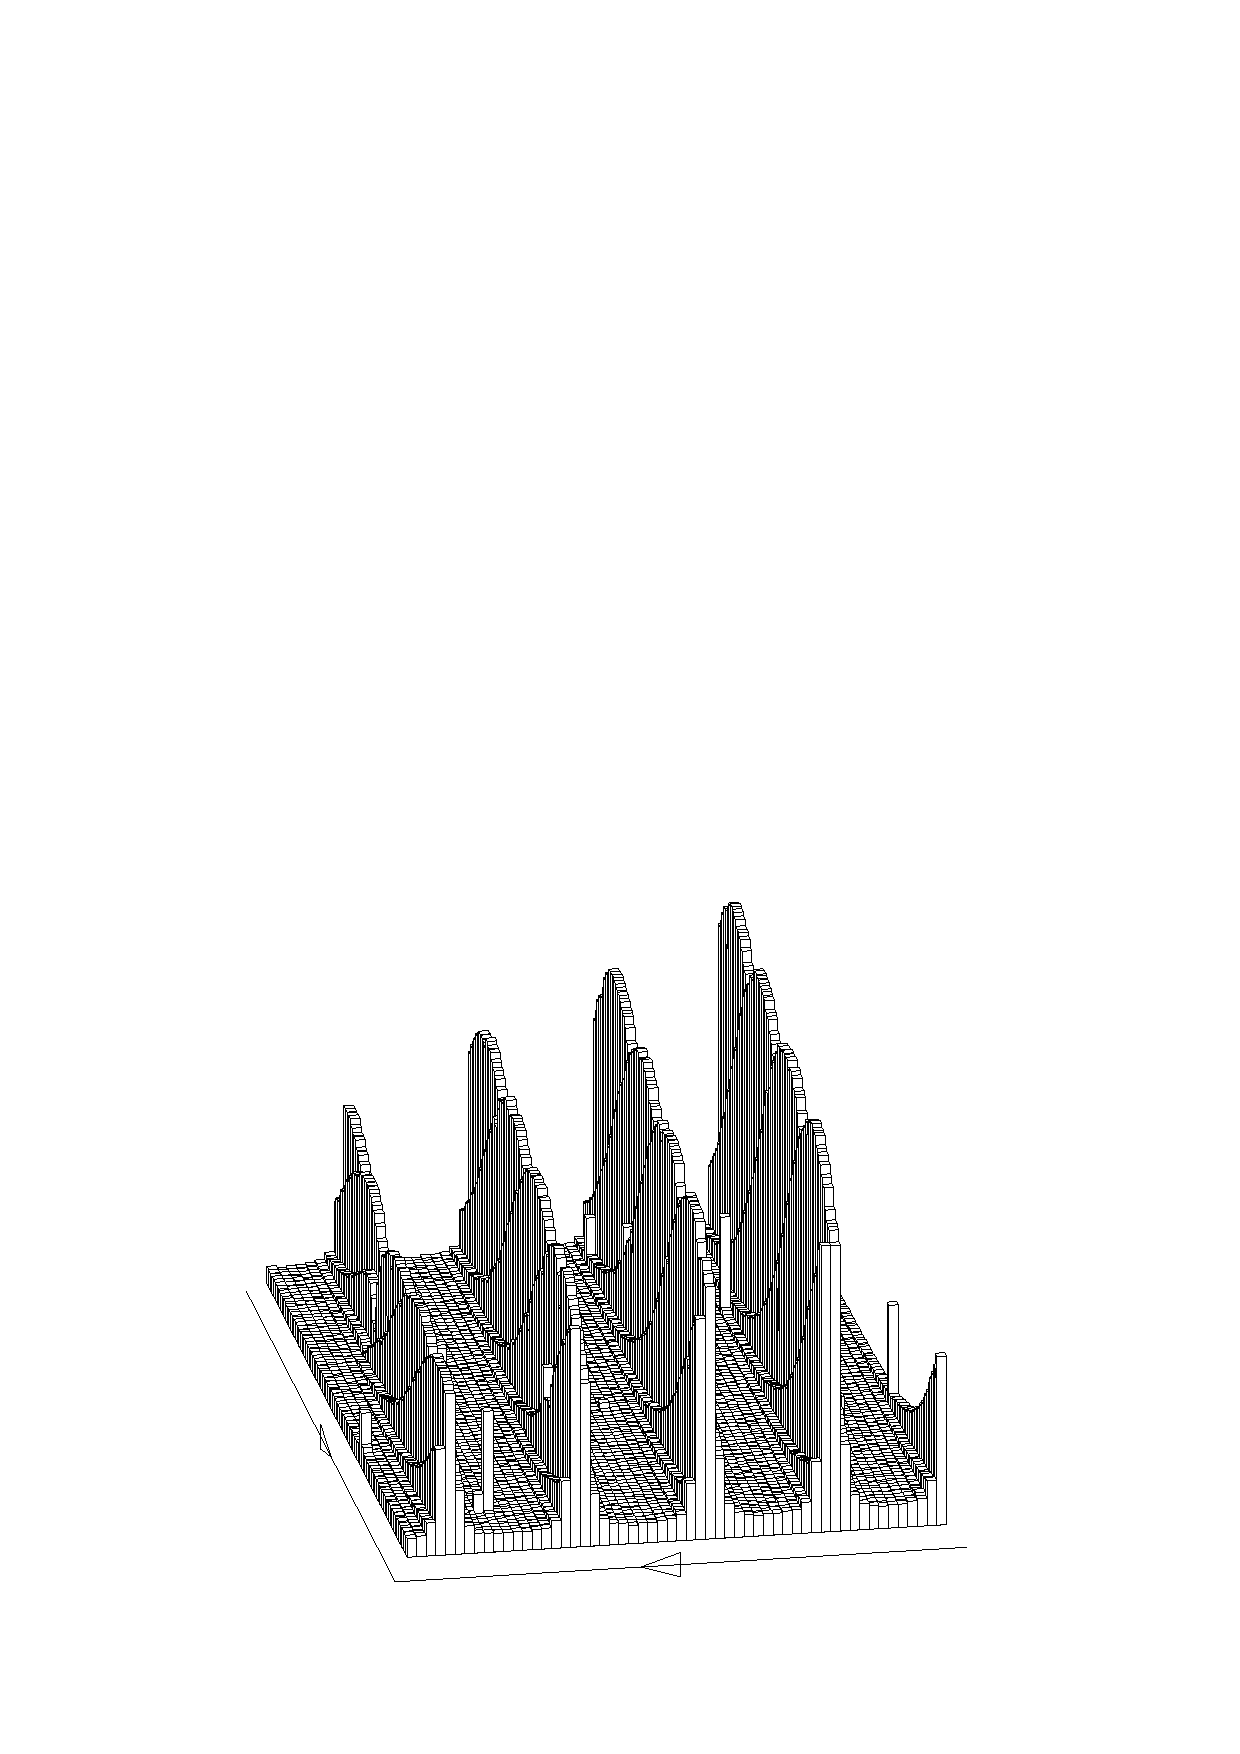
\includegraphics[height=120mm]{sg9_cover}

   An Echelle spectrum
   \end{center}
% ? End of picture

% ? Heading for abstract if used.
%  \vspace{10mm}
%  \begin{center}
%     {\Large\bf Abstract}
%  \end{center}
% ? End of heading for abstract.
\end{latexonly}

%  HTML documentation header.
%  ==========================
\begin{htmlonly}
   \xlabel{}
   \begin{rawhtml} <H1> \end{rawhtml}
      \stardoctitle\\
%     \stardocversion\\
%     \stardocmanual
   \begin{rawhtml} </H1> \end{rawhtml}

% ? Add picture here if required.
   \begin{figure}[h]
   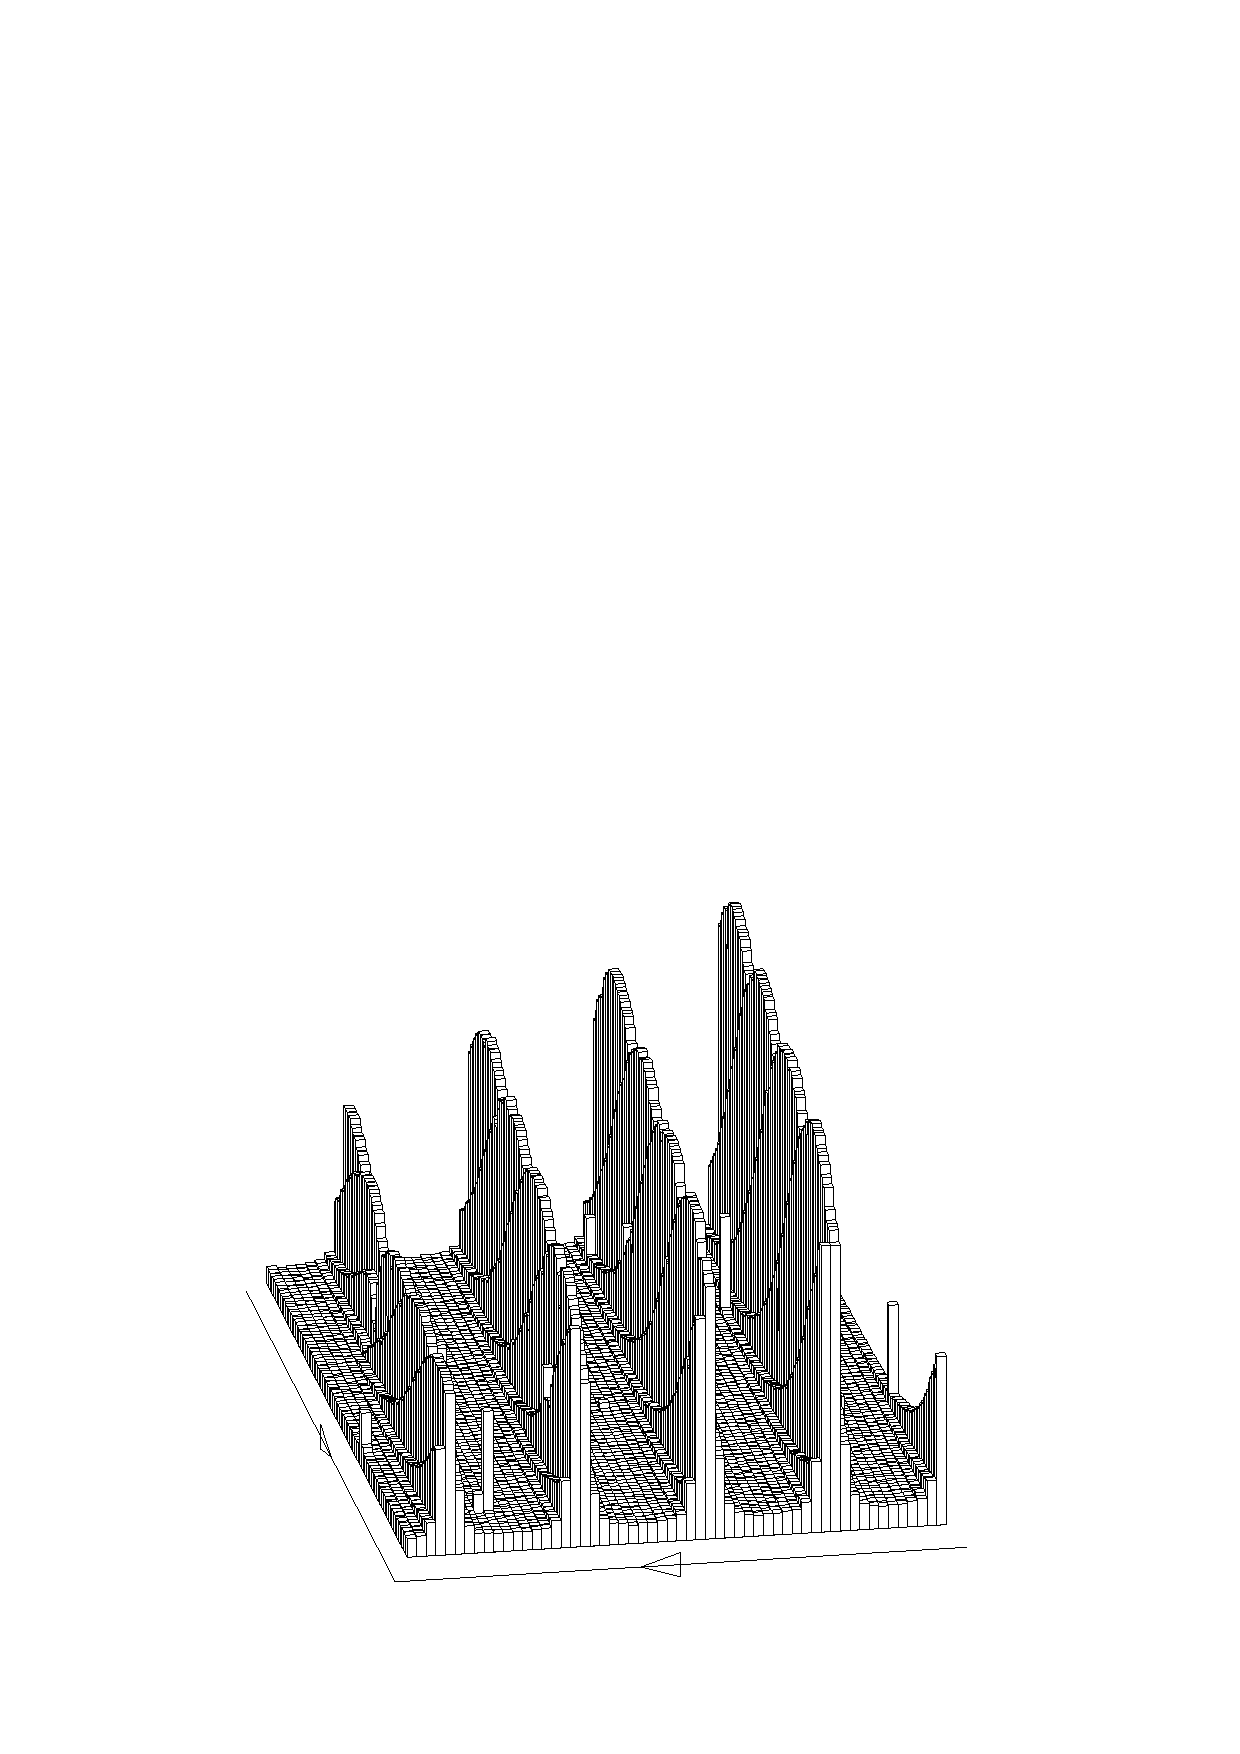
\includegraphics[height=120mm]{sg9_cover}
   \end{figure}

   \begin{center}
   An Echelle spectrum
   \end{center}

% ? End of picture.

   \begin{rawhtml} <P> <I> \end{rawhtml}
   \stardoccategory\ \stardocnumber \\
   \stardocauthors \\
   \stardocdate
   \begin{rawhtml} </I> </P> <H3> \end{rawhtml}
      \htmladdnormallink{CCLRC}{http://www.cclrc.ac.uk} /
      \htmladdnormallink{Rutherford Appleton Laboratory}
                        {http://www.cclrc.ac.uk/ral} \\
      \htmladdnormallink{Particle Physics \& Astronomy Research Council}
                        {http://www.pparc.ac.uk} \\
   \begin{rawhtml} </H3> <H2> \end{rawhtml}
      \htmladdnormallink{Starlink Project}{http://www.starlink.ac.uk/}
   \begin{rawhtml} </H2> \end{rawhtml}
   \htmladdnormallink{\htmladdimg{source.gif} Retrieve hardcopy}
      {http://www.starlink.ac.uk/cgi-bin/hcserver?\stardocsource}\\

%  HTML document table of contents.
%  ================================
%  Add table of contents header and a navigation button to return to this
%  point in the document (this should always go before the abstract \section).
  \label{stardoccontents}
  \begin{rawhtml}
    <HR>
    <H2>Contents</H2>
  \end{rawhtml}
  \newcommand{\latexonlytoc}[0]{}
  \htmladdtonavigation{\htmlref{\htmladdimg{contents_motif.gif}}
        {stardoccontents}}

% ? New section for abstract if used.
% \section{\xlabel{abstract}Abstract}
% ? End of new section for abstract
\end{htmlonly}

% -----------------------------------------------------------------------------
% ? Document Abstract. (if used)
%  ==================
% \stardocabstract
% ? End of document abstract
% -----------------------------------------------------------------------------
% ? Latex document Table of Contents (if used).
%  ===========================================
 \newpage
 \begin{latexonly}
   \setlength{\parskip}{0mm}
   \markboth{Contents}{\stardocname}
   \latexonlytoc
   \setlength{\parskip}{\medskipamount}
 \end{latexonly}
% ? End of Latex document table of contents
% -----------------------------------------------------------------------------
%%%%%%%%%%%%%%%%%%%%%%%%%%%%%%%%%%%%%%%%%%%%%%%%%%%%%%%%%%%%%%%%%%%%%%%%%%%
\newpage
\renewcommand{\thepage}{\arabic{page}}
\setcounter{page}{1}

\section{\label{se_introduction}\xlabel{introduction}Introduction}
\markboth{Introduction}{\stardocname}

\htmlref{{\bf Echelle}}{gl_echelle} \htmlref{{\bf
spectrographs}}{gl_spectrograph} are available as
common-user instruments at several observatories and satellites.  These
spectrographs offer the observer both a reasonably high
\htmlref{{\bf resolution}}{gl_resolution} and
a wide wavelength-coverage; at the expense of a fairly complex
data-reduction procedure.

This document is intended as an introductory guide for observers
new to \'{e}chelle work.  Experienced observers may wish to consult
\sgspec{\S \ref{se_facilities} for outline information}
{the \htmlref{outline information}{se_facilities}}
on the main packages available for \'{e}chelle data reduction.


\subsection{\label{se_other_sources}\xlabel{other_sources}Other
            Sources of Information}

This Guide complements the Starlink \xref{{\sl Echelle Data Reduction
Cookbook} (Starlink document SC/3)}{sc3}{} which contains examples of
data-reduction scripts, including templates for fully automated data
reductions with \xref{ECHOMOP}{sun152}{}\@.

A significant part of the process of successful spectrum extraction
is the preliminary handling of the \htmlref{{\bf CCD}}{gl_ccd} data frames.
Those planning to use
\htmladdnormallink{IRAF}
{http://www.starlink.ac.uk/iraf/web/iraf-homepage.html}\sgspec{\footnote{IRAF
documents can be found in your IRAF installation; you
do not need to get them from Tucson or a mirror.  Check with your manager for
details.}}{{\em (All IRAF-related hyperlinks in this document are to the
UK-based Starlink IRAF mirror except \htmladdnormallink{this one}
{http://iraf.noao.edu/} which goes to the Tucson site.)}} should consult
\htmladdnormallink{{\sl A User's Guide to CCD Reductions with IRAF}}
{ftp://starlink-ftp.rl.ac.uk/pub/iraf/iraf/docs/ccduser2.ps.Z} (UGCRI) by Philip Massey.
UGCRI is quite a good document for {\em any} user of CCD data, even those
planning to use {\em e.g.} \xref{CCDPACK}{sun139}{} or
\xref{FIGARO}{sun86}{} to do the preparation\sgspec{---}{ - }the
\xref{{\sl CCD Reduction Cookbook} (SC/5)}{sc5}{} is the definitive
introduction to this type of work.

IRAF users should look at the two documents for \'{e}chelle data reduction
within IRAF:
\htmladdnormallink{{\sl A User's Guide to Reducing Echelle Spectra With IRAF}}
{ftp://starlink-ftp.rl.ac.uk/pub/iraf/iraf/docs/ech.ps.Z}, and
\htmladdnormallink{{\sl Guide to the Slit Spectra Reduction Task DOECSLIT.}}
{ftp://starlink-ftp.rl.ac.uk/pub/iraf/iraf/docs/doecslit.ps.Z}
These give a comprehensive description of the IRAF approach to \'{e}chelle
data.  There is also a hypertext tutorial for DOECSLIT at

\begin{itemize}

\item \htmladdnormallink{{\tt
      http://www.starlink.ac.uk/iraf/web/tutorials/doecslit/doecslit.html}}
      {http://www.starlink.ac.uk/iraf/web/tutorials/doecslit/doecslit.html}

\end{itemize}

You may be able to access a local copy of this tutorial; consult your
system manager.

There is an excellent guide tailored to the reduction of \'{e}chelle
data taken using the Hamilton Spectrograph:
\htmladdnormallink{{\sl Introduction to Echelle
Data Reduction  Using the Image Reduction Analysis Facility,}}
{http://www.star.ucl.ac.uk/\~{}mjc/echelle/misc/LickTech74.ps.gz} which is a
Lick Observatory Technical report\@.
\begin{latexonly}
(A PostScript copy is available from the Starlink Echelle Support
Pages.)
\end{latexonly}
This is a complete
step-by-step run through of \'{e}chelle data reduction using
IRAF\sgspec{---}{ - }from CCD data to calibrated spectra.

The primary documentation for ECHOMOP is in \xref{{\sl
ECHOMOP\sgspec{---}{ - }Echelle
data reduction package} (Starlink document SUN/152)}{sun152}{}\@.
This document explains each of the data-reduction steps using ECHOMOP and
includes some general advice and tips.
There is also additional information and advice in the on-line HELP for
ECHOMOP if you get stuck.

An up-to-date set of hypertext documents for Starlink \'{e}chelle data
reduction and related information; including hypertext help, bug
reports, comments and news, is maintained at

\begin{itemize}

\item \sgspec{{\tt http://www.star.ucl.ac.uk/\symbol{126}mjc/echelle/}}
      {\htmladdnormallink{\verb+http://www.star.ucl.ac.uk/~mjc/echelle/+}
      {http://www.star.ucl.ac.uk/\~{}mjc/echelle/}}

\end{itemize}

Terms in the body text of this Guide in {\bf bold} are described in the
\htmlref{glossary}{se_glossary} later in this document;
if you cannot find the term you want there, you might try the
{\sl NASA Thesaurus:}

\begin{itemize}

\item \sgspec{{\tt http://www.sti.nasa.gov/nasa-thesaurus.html}}
      {\htmladdnormallink{\verb+http://www.sti.nasa.gov/nasa-thesaurus.html+}
      {http://www.sti.nasa.gov/nasa-thesaurus.html}}

\end{itemize}


%%%%%%%%%%%%%%%%%%%%%%%%%%%%%%%%%%%%%%%%%%%%%%%%%%%%%%%%%%%%%%%%%%%%%%%%%%%
\section{\label{se_example_echelle}\xlabel{example_echelle}An Echelle
         Spectrum}\markboth{An Echelle Spectrum}{\stardocname}

In `traditional' spectrographs a dispersing element\sgspec{---}{ - }typically a
\htmlref{{\bf diffraction grating}}{gl_grating} or
\htmlref{{\bf prism}}{gl_prism}\sgspec{---}{ - }is used to produce the spectrum.
This results in a single spectrum which can be imaged using a
\htmlref{{\bf CCD}}{gl_ccd} or other
type of camera.  The data can then be extracted using a suitable
program.  The recordable part of the wavelength range covered by this type of
spectrograph is limited by the size of available image sensors,
{\em i.e.}, CCDs.

A quick inspection of a CCD image of such a spectrum will also reveal
that much of the detector area away from the spectrum itself is unused.
One method of optimising the use of the available detector area is to
use an \'{e}chelle spectrograph.

An \'{e}chelle is a diffraction grating in which the rulings are much
further apart than usual.
This leads to spectra of very high \htmlref{{\bf dispersion}}{gl_dispersion},
but only over a short wavelength range in each order.
As well as being `short', the high orders will overlap.  To overcome
this effect a \htmlref{{\bf cross-dispersing}}{gl_cross_dispersion}
element is used to produce an
\htmlref{{\bf order separation}}{gl_order_separation}.
\sgspec{Figure~\ref{fi_ech_image}}{The figure below}
shows a small part of such
an \'{e}chellogram recorded with a CCD camera.  You can see a short part
of three orders which run from the top to the bottom of the image at a
slight angle.  In the order to the right you can see a couple of
absorption features.  Several \htmlref{{\bf cosmic-ray events}}{gl_cosmic_ray}
(bright spots) are also visible.

\begin{figure}
\begin{center}
\sgspec{\leavevmode
\includegraphics[height=105mm]{sg9_04}}
{\leavevmode
\includegraphics[height=136mm]{sg9_04}}

\parbox{140mm}{
\caption{Echelle Image: Part of an \'{e}chelle image produced with UCLES
         and a CCD camera.}
\label{fi_ech_image}
}
\end{center}
\end{figure}

Echelle spectrographs for astronomy are designed so that the wavelength
coverage in one order will overlap the coverage of the adjacent orders.
(That is at least for the middle orders in the full
\'{e}chellogram\sgspec{---}{ - }there
may be some gaps at the extremes of the image.)  Using a suitable
detector\sgspec{--}{-}usually a CCD\sgspec{---}{ - }these spectral
orders can be recorded.

The extraction of an \'{e}chelle spectrum from a set of images is, in
principle, similar to the extraction of a single-order spectrum.
Additional complexity arises because:

\begin{itemize}

\item There are more data to extract.

\item The orders can have a more complex shape than those from a
      single-order instrument.

\item The high \htmlref{{\bf dispersion}}{gl_dispersion} used can make
      it difficult to distinguish
      between true spectral features and cosmic-ray events.

\item \htmlref{{\bf Flat fielding}}{gl_flat_field} the data can be difficult.

\item In some cases adjacent orders overlap slightly in the spatial
      direction (there can be several reasons for this) making
      accurate background subtraction difficult.

\end{itemize}

Fortunately, there are several dedicated software packages available
which address these specific features of \'{e}chelle data reduction.

%%%%%%%%%%%%%%%%%%%%%%%%%%%%%%%%%%%%%%%%%%%%%%%%%%%%%%%%%%%%%%%%%%%%%%%%%%%
\section{\label{se_preparation}\xlabel{preparation}Preparing for Observation}
\markboth{Preparing for Observation}{\stardocname}

There is a comprehensive Starlink Guide for those preparing for
an observing run\sgspec{---}{ - }\xref{{\sl Preparing to Observe}
(Starlink document SG/10)}{sg10}{}.

In this section some notes on what to be aware of prior to an observing
run are given.
In outline: to successfully extract and calibrate an \'{e}chelle spectrum
a complete set of reference frames should be obtained at the telescope.

You might want to refer to the more extensive discussion of CCD data
calibration in: {\sl A User's guide to CCD Reductions with IRAF,} the
section entitled ``How Many and What Calibration Frames Do You Need?''


\subsection{What CCD Data Do You Need?}

This is what you need to attempt `textbook' \'{e}chelle
data preparation:

\begin{description}

\item [{\bf Bias frames}]
      Zero-second exposures taken with no signal light entering the
      instrument but with any pre-flash used for the object exposures
      present.

\item [{\bf Dark frames}]
      Long exposures taken with the shutter closed.  Typically, the
      exposure time used is similar to that selected for the object
      frames.

\item [{\bf Flat-field frames}]
      Exposures taken with a suitable continuum lamp
      (usually Tungsten) as light source.

\item [{\bf Arc frames}]
      Exposures taken with an \htmlref{{\bf arc lamp}}{gl_arc}
      (usually Thorium-Argon) as
      light source, to be used for wavelength reference.

\item [{\bf Object frames}]
      Exposures taken with a target object or reference object as the
      `light source'.

\end{description}

The arc and object frames will be processed by the \'{e}chelle data
reduction software.  The bias and flat-field frames are used in the
preparation of the CCD data.


\subsection{Detector Pre-processing}

A more complete introduction to the handling of \htmlref{{\bf CCD}}{gl_ccd}
data can be found in the \xref{{\sl CCD Reduction Cookbook} (SC/5)}{sc5}{},
a brief outline is given here.

In order to remove detector-related effects a complete set of
\htmlref{{\bf bias}}{gl_bias_frame}, \htmlref{{\bf dark}}{gl_dark_frame},
and
\htmlref{{\bf flat-field}}{gl_flat_field} frames should be obtained.
It is important to {\em
\htmlref{{\bf bracket}}{gl_bracketing}} the science data exposures with
complete sets of CCD
characterisation frames.  A post-observation review of these will reveal
any image shifts.  Having bracket frames allows the data to be
accurately prepared even in the event that some time-dependent variation
is found (as long as its a small, slow-varying effect).

See \sgspec{\S \ref{se_image_preparation}}
{\htmlref{{\sl Image Preparation}}{se_image_preparation}}
for outline details of CCD data preparation.

In some cases it may be possible to not use any
\htmlref{{\bf bias frames}}{gl_bias_frame}.  Instead,
a median value for the bias level is obtained by inspecting the
\htmlref{{\bf overscan region}}{gl_overscan} in some or all of the object/arc
frames.
You can use fewer bias frames when you have a high signal-to-detector-noise
ratio.

For exposure times limited by cosmic-ray event counts, the
\htmlref{{\bf dark current}}{gl_dark_current}
in most CCD cameras is not a significant factor.  The simplest way to
decide whether to take dark frames is to take one of exposure time
similar to that you are using for object frames, and check the signal level.


\subsection{\label{se_flat_beware}\xlabel{flat_beware}Flat Fields}

Beware of flat fielding in \'{e}chelle spectroscopy.  For a stable
spectrograph ({\em{e.g.}} \htmlref{{\bf UCLES}}{gl_ucles} which is in the
\htmlref{{\bf AAT}}{gl_aao_aat} coud\'{e} room)
you can take flat-field frames at any suitable time.  For less-stable
instruments it may be difficult to get a useable flat field.
The problem is getting the object and flat-field orders to fall on the
detector in the same place.
In this case, the best procedure is to take flat fields immediately
before and after each science exposure in the same way as you would
take arcs.

When preparing flat-field frames for your data ensure that a
\htmlref{{\bf dekker}}{gl_dekker} size (length)
larger than that used for the science exposures is used\sgspec{---}{ - }avoid
order overlap in the image, though.  This ensures that a reasonable
\htmlref{{\bf flat-field}}{gl_flat_field} is available across the complete
profile of each order.  If a choice of gratings is available, use the
one which will give you the widest order separation.

In some areas of the \'{e}chellogram the brightness of a single
flat-field may fall off or vary rapidly due to the characteristic
spectrum of the \htmlref{{\bf arc lamp}}{gl_arc}
used or variations in the efficiency of the
detector (some front-illuminated CCDs have 20\sgspec{--}{-}30\%
variations in efficiency over a small wavelength band).
There are two ways to overcome these effects: use a different lamp
to produce the flat field in those orders\sgspec{---}{ - }but usually a
different lamp is not available\sgspec{---}{ - }or, obtain as many
unsaturated flat fields as possible and sum or average them.

It may not always be necessary to flat field; a flat-field frame
taken with a modern CCD can be flat in response to only a few percent.
You may only need to flat field if the signal-to-noise ratio you
require is particularly high.  The precise figures will depend upon
several factors, and should be estimated for each science object.


\subsection{Order Tracing}

Accurate determination of the path of the \'{e}chelle orders across the
images is vital to achieving the best extractions.  Processing software
requires a bright, clean ({\em{i.e.}}, cosmic-ray free) image from which
to trace the orders.

For well-exposed continuous spectra the object frame can be used for
tracing.  However, in the case of faint objects, or
objects with strong absorption features in their spectra, tracing of
object frames will not be easy.
A \htmlref{{\bf flat-field frame}}{gl_flat_field} can be used for tracing as
this is likely to give a good signal.
Therefore, if necessary, obtain a few flat fields with a narrow
\htmlref{{\bf dekker}}{gl_dekker} to improve the traces.
It may be worth having {\em several} possible frames for
tracing\sgspec{---}{ - }in case some of them are badly contaminated
by cosmic rays and so difficult to use.


\subsection{Wavelength Calibration}

As with the CCD characterisation frames, wavelength-scale reference
(arc) frames should be taken \htmlref{{\bf bracketing}}{gl_bracketing} the
science exposures {\em if} precise wavelength scales are required.
At the high \htmlref{{\bf dispersions}}{gl_dispersion}
used in \'{e}chelle spectrographs a small
change in the optical system can lead to a detectable shift between the
bracketing images.
Using both arc spectra, a time-weighted mean wavelength scale can be
produced and applied to the science data.


\subsection{Flux Calibration}

Existing standard star data is often based upon a system in which the
band size is much larger than the wavelength coverage of
a single \'{e}chelle order.  In practice, this can make the application
of proper flux calibration to high-resolution \'{e}chelle spectra
difficult or infeasible.  Proper high-resolution spectral standards are
now starting to become available (notably for \htmlref{{\bf HST}}{gl_hst})\@.
If you intend to flux calibrate your data you should ensure that suitable
standards are available.

Refer to \sgspec{\S \ref{se_finishing}}{\htmlref{{\sl{Finishing}}}
{{se_finishing}}} for more information on the problems associated with
flux calibration.

%%%%%%%%%%%%%%%%%%%%%%%%%%%%%%%%%%%%%%%%%%%%%%%%%%%%%%%%%%%%%%%%%%%%%%%%%%%
\section{\label{se_basics}\xlabel{basics}The Basics of Echelle Data Reduction}
\markboth{The Basics of Echelle Data Reduction}{\stardocname}

\begin{htmlonly}
The flow chart below maps out the main steps in the
\'{e}chelle data reduction process.
\begin{rawhtml}
<PRE>
                     raw CCD
                        |
                        v
                  CCD  processing
                        |
                        v
                  prepared images
                        |
                        v
                  order  location
                        |
                        v
                   order tracing
                        |
                        v
                    slit set-up
                        |
                        v
                     normalise
                    flat  field
                        |
                        v
       /---------choose background---------\
       |                                   |
scattered light                      sky  subtract
       |                                   |
       v                                   v
     model                             model sky
scattered light                            |
       |                                   |
       \-------->background  model<--------/
                        |
                        V
                     extract
                        |
       /----------------+------------------\
       |                                   |
      arcs                              objects
       |                                   |
       v                                   |
locate arc lines                           |
       |                                   |
       v                                   |
 fit wavelength                            |
     scales                                |
       |                                   |
       \---------->wavelength-<------------/
               calibrated  objects
                        |
                        +------------->single-order spectra
                        |
       /----------------+------------------\
       |                |                  |
       v                |                  v
 blaze correct          |           flux calibrate
       |                v                  |
       \---------->scrunch/merge<----------/
                        |
                        v
                  merged spectra
</PRE>
\end{rawhtml}
\end{htmlonly}

\sgspec{Figure~\ref{fi_flow} is a flow chart which maps out the main steps
in the \'{e}chelle data reduction process.}{}
\xref{ECHMENU}{sun152}{ECHMENU} is a menu-driven program in which each of
the natural steps in the reduction process is handled by a task.
This is the top-level menu presented by ECHMENU:

\begin{latexonly}
\begin{verbatim}
  0. HELP/HYPER (ASCII or hypertext help).
  1. Start a reduction.                 16. Check trace consistency.
  2. Trace orders.                      17. Post-trace Cosmic Ray locate.
  3. Clip fitted traces.                18. Image cosmic ray pixels.
  4. Determine dekker/object extent.    19. Quick-look Extraction.
  5. Model flat field.                  20. Check wavelength scales.
  6. Model sky.                         21. Scrunch and merge multiple.
  7. Model object profile.              22. Model scattered light.
  8. Extract orders 1-D.                23. ADJUST tuning parameters.
  9. Locate arc line candidates.        24. Set single-order operations.
 10. Identify features.                 25. Set all-order operations.
 11. Flatten order shape.               26. DISABLE an order.
 12. Scrunch to linear scale.           27. PLOT reduction arrays.
 13. Model/Extract orders 2-D.          28. Full MENU.
 14. Save reduced data.                 29. System ($) commands.
 15. Plot order traces.                 30. Output balance-factor frame.
                                        31. EXIT (alias Q/E/QUIT/EXIT/99).
\end{verbatim}
\end{latexonly}
\begin{htmlonly}
\begin{rawhtml}
<PRE WIDTH=80>
  <A HREF="/sun152.htx/#xref_option0">0.</A> HELP/HYPER (ASCII or hypertext help).
  <A HREF="/sun152.htx/#xref_option1">1.</A> Start a reduction.                 <A HREF="/sun152.htx/#xref_option16">16.</A> Check trace consistency.
  <A HREF="/sun152.htx/#xref_option2">2.</A> Trace orders.                      <A HREF="/sun152.htx/#xref_option17">17.</A> Post-trace Cosmic Ray locate.
  <A HREF="/sun152.htx/#xref_option3">3.</A> Clip fitted traces.                <A HREF="/sun152.htx/#xref_option18">18.</A> Image cosmic ray pixels.
  <A HREF="/sun152.htx/#xref_option4">4.</A> Determine dekker/object extent.    <A HREF="/sun152.htx/#xref_option19">19.</A> Quick-look Extraction.
  <A HREF="/sun152.htx/#xref_option5">5.</A> Model flat field.                  <A HREF="/sun152.htx/#xref_option20">20.</A> Check wavelength scales.
  <A HREF="/sun152.htx/#xref_option6">6.</A> Model sky.                         <A HREF="/sun152.htx/#xref_option21">21.</A> Scrunch and merge multiple.
  <A HREF="/sun152.htx/#xref_option7">7.</A> Model object profile.              <A HREF="/sun152.htx/#xref_option22">22.</A> Model scattered light.
  <A HREF="/sun152.htx/#xref_option8">8.</A> Extract orders 1-D.                <A HREF="/sun152.htx/#xref_option23">23.</A> ADJUST tuning parameters.
  <A HREF="/sun152.htx/#xref_option9">9.</A> Locate arc line candidates.        <A HREF="/sun152.htx/#xref_option24">24.</A> Set single-order operations.
 <A HREF="/sun152.htx/#xref_option10">10.</A> Identify features.                 <A HREF="/sun152.htx/#xref_option25">25.</A> Set all-order operations.
 <A HREF="/sun152.htx/#xref_option11">11.</A> Flatten order shape.               <A HREF="/sun152.htx/#xref_option26">26.</A> DISABLE an order.
 <A HREF="/sun152.htx/#xref_option12">12.</A> Scrunch to linear scale.           <A HREF="/sun152.htx/#xref_option27">27.</A> PLOT reduction arrays.
 <A HREF="/sun152.htx/#xref_option13">13.</A> Model/Extract orders 2-D.          <A HREF="/sun152.htx/#xref_option28">28.</A> Full MENU.
 <A HREF="/sun152.htx/#xref_option14">14.</A> Save reduced data.                 <A HREF="/sun152.htx/#xref_option29">29.</A> System ($) commands.
 <A HREF="/sun152.htx/#xref_option15">15.</A> Plot order traces.                 <A HREF="/sun152.htx/#xref_option30">30.</A> Output balance-factor frame.
                                        31. EXIT (alias Q/E/QUIT/EXIT/99).
</PRE>
\end{rawhtml}
\end{htmlonly}

\begin{latexonly}
\begin{figure}
\begin{center}
\setlength{\unitlength}{1cm}
\begin{picture}(15,20)(-2.5,0)
    \tiny

    \echdiagobjectbox{5.0}{20.25}{raw CCD}
    \put(5.0, 20.0){\vector(0,-1){0.5}}
    \echdiagactionbox{4.0}{19.0}{CCD processing}
    \put(5.0, 19.0){\vector(0,-1){0.5}}
    \echdiagobjectbox{5.0}{18.25}{prepared images}
    \put(5.0, 18.0){\vector(0,-1){0.5}}
    \echdiagactionbox{4.0}{17.0}{order location}
    \put(5.0, 17.0){\vector(0,-1){0.5}}
    \echdiagactionbox{4.0}{16.0}{order tracing}
    \put(5.0, 16.0){\vector(0,-1){0.5}}
    \echdiagactionbox{4.0}{15.0}{slit set-up}
    \put(5.0, 15.0){\vector(0,-1){0.5}}
    \echdiagactionbox{4.0}{14.0}{normalise\\flat field}
    \put(5.0, 14.0){\vector(0,-1){0.5}}
    \echdiagactionbox{4.0}{13.0}{choose\\background}

    \put(4.0, 13.25){\line(-1,0){1.5}}
    \put(2.5, 13.25){\line(0,-1){0.75}}
    \echdiagarmtext{2.5}{12.25}{scattered light}
    \put(2.5, 12.0){\vector(0,-1){0.5}}
    \echdiagactionbox{1.5}{11.0}{model\\scattered light}
    \put(2.5, 11.0){\line(0,-1){0.75}}
    \put(2.5, 10.25){\vector(1,0){1.5}}

    \put(6.0, 13.25){\line(1,0){1.5}}
    \put(7.5, 13.25){\line(0,-1){0.75}}
    \echdiagarmtext{7.5}{12.25}{sky subtract}
    \put(7.5, 12.0){\vector(0,-1){0.5}}
    \echdiagactionbox{6.5}{11.0}{model\\sky}
    \put(7.5, 11.0){\line(0,-1){0.75}}
    \put(7.5, 10.25){\vector(-1,0){1.5}}

    \echdiagobjectbox{5.0}{10.25}{background\\model}
    \put(5.0, 10.0){\vector(0,-1){0.5}}
    \echdiagactionbox{4.0}{9.0}{extract}
    \put(5.0, 9.0){\line(0,-1){0.25}}
    \put(2.5, 8.75){\line(1,0){5.0}}

    \put(2.5, 8.75){\line(0,-1){0.25}}
    \echdiagarmtext{2.5}{8.25}{arcs}
    \put(2.5, 8.0){\vector(0,-1){0.5}}
    \echdiagactionbox{1.5}{7.0}{locate arc lines}
    \put(2.5, 7.0){\vector(0,-1){0.5}}
    \echdiagactionbox{1.5}{6.0}{fit wavelength\\scales}
    \put(2.5, 6.0){\line(0,-1){0.75}}
    \put(2.5, 5.25){\vector(1,0){1.5}}

    \put(7.5, 8.75){\line(0,-1){0.25}}
    \echdiagarmtext{7.5}{8.25}{objects}
    \put(7.5, 8.0){\line(0,-1){2.75}}
    \put(7.5, 5.25){\vector(-1,0){1.5}}

    \echdiagobjectbox{5.0}{5.25}{wavelength\\calib'd objects}
    \put(5.0, 5.0){\vector(0,-1){2.5}}
    \put(5.0, 4.75){\vector(1,0){3.0}}
    \echdiagobjectbox{9.0}{4.75}{single-order\\spectra}
    \put(2.5, 4.25){\line(1,0){5.0}}

    \put(2.5, 4.25){\vector(0,-1){0.75}}
    \echdiagactionbox{1.5}{3}{blaze correct}
    \put(2.5, 3.0){\line(0,-1){0.75}}
    \put(2.5, 2.25){\vector(1,0){1.5}}

    \put(7.5, 4.25){\vector(0,-1){0.75}}
    \echdiagactionbox{6.5}{3}{flux calibrate}
    \put(7.5, 3.0){\line(0,-1){0.75}}
    \put(7.5, 2.25){\vector(-1,0){1.5}}

    \echdiagactionbox{4.0}{2}{scrunch/merge}
    \put(5.0, 2.0){\vector(0,-1){0.5}}
    \echdiagobjectbox{5.0}{1.25}{merged spectra}

\end{picture}
\parbox{140mm}{
\caption{Outline of the \'{e}chelle data reduction process.}
\label{fi_flow}
}
\end{center}
\end{figure}
\end{latexonly}

In this section each of the major steps is outlined and some of the
important and perhaps tricky considerations are mentioned.
Most of the steps are similar to those which would be used for
extraction of a single-order spectrum, plus a few additional elements
to deal with the multiple orders.
The handling of cosmic-ray removal is described separately at the end of
this section as there are several different approaches to the problem.


\subsection{\label{se_image_preparation}\xlabel{image_preparation}Image
            Preparation}

Most \'{e}chelle data will be obtained using a CCD to record the
image.  Careful preparation of the CCD data prior to attempting
extraction of spectra is essential.  In this Guide the basic
procedures are outlined (very!) briefly.  Those points relevant to
\'{e}chelle data reduction are included.

The basic steps in the preparation are:

\begin{description}

\item [{\bf Generate \htmlref{bias frame}{gl_bias_frame}}]
      Typically done by finding the median of several frames taken at
      the telescope.

\item [{\bf Generate \htmlref{flat-field frame}{gl_flat_field}}]
      Again, done by finding the median of several frames taken at
      the telescope.  Before taking the median of the frames, the
      median bias frame and a zero-offset constant are subtracted
      (see below).

\item [{\bf Subtract bias frame}]
      The median bias frame is subtracted from each arc frame and
      each object frame.

\item [{\bf Subtract zero-offset}]
      A selected area of the CCD \htmlref{{\bf overscan region}}{gl_overscan}
      is used to find the
      `zero-level' of the camera electronics.  This is usually a number
      in the range 20\sgspec{--}{-}200 \htmlref{{\bf ADU}}{gl_adu}\@.
      The median value of the selected region
      should be used (to avoid cosmic-ray contamination).  This constant
      value is then subtracted from every pixel in the CCD image.

\item [{\bf Crop images}]
      Regions\sgspec{---}{ - }such as the overscan\sgspec{---}{ - }are
      not used during the extraction
      process and should be removed (the same as cropping a photograph)
      as they may confuse some of the algorithms in the \'{e}chelle data
      reduction engine.  Very often CCD images will have `rough' edges,
      {\em i.e.} non-useable data, which should also be trimmed off at
      this point.

\end{description}

Depending on your source data and choice of reduction software you may
need to:

\begin{description}

\item [{\bf Rotate and orient the image}]
      All the major packages constrain the orientation of the \'{e}chelle
      orders in some way.  The images may have to be adjusted to meet
      these constraints.
      In general, if the \'{e}chelle orders in your data run roughly
      horizontally (parallel to the X-axis) and the wavelength increases
      from left to right you will be alright.
      In other situations, you may need to use some image utilities to
      re-orient the data.
      This may involve rotating and perhaps reflecting the images.

\end{description}

You may have data which contain `dead columns' or few-pixel hot-spots.
Handling of these is discussed in the documentation for the CCD data
preparation packages.

Once the set of arc and object images have been prepared in this way the
\'{e}chelle data reduction process can begin.


\subsubsection{Software for CCD Data Preparation}

There are quite a few different packages for preparing CCD data. All
these packages offer similar functionality.  You'll probably find that
it's easiest to use the preparation package which complements the
\'{e}chelle reduction software you choose, {\em e.g.}, {\tt
noao.imred.ccdred} for IRAF {\tt doecslit}\@.  There are two popular
Starlink packages which you might use,
\xref{FIGARO}{sun86}{} and \xref{CCDPACK}{sun139}{}\@.  CCDPACK includes
some tools for conveniently managing the preparation of many frames and
supports error propagation.


\subsection{\label{se_order_location}\xlabel{order_location}Order Location}

Order location is simply the process of finding the approximate position
of each of the orders in an \'{e}chelle image.  You can select which of the
located orders should then be extracted.  This saves time if there is no
useful data in some of the orders.  Location is achieved by taking a
slice across the dispersion direction which when plotted appears similar
to the graph \sgspec{in Figure~\ref{fi_scan_plot}\@.}{below.}

This example is a section across an \htmlref{{\bf IUE}}{gl_iue} \'{echelle}
image.
You can see about 60 orders are present in this case.
In practice, the section across the image will use data from several
columns (in the case of a roughly horizontal dispersion), rather than
a single column.

\begin{figure}
\begin{center}
\sgspec{\leavevmode
\includegraphics[height=105mm]{sg9_01}}
{\leavevmode
\includegraphics[height=136mm]{sg9_01}}

\parbox{140mm}{
\caption{Order Location: cross-dispersion section through an IUE
         \'{e}chelle spectrum.}
\label{fi_scan_plot}
}
\end{center}
\end{figure}


\subsection{\label{se_order_tracing}\xlabel{order_tracing}Order Tracing}

Once the required orders have been selected the next step is to
determine the path of each of them across the image.  This process is {\sl
order tracing.}  Typically the tracing procedure will involve sampling
each order in steps along the dispersion direction.  The reduction
program will attempt to estimate the centre of the order at each sample
point.  Once an order has been traced in this way you will have the
option to fit a curve to the sample data.  If all is well, the curve
should represent the true path of the order across the frame.  In
practice, some of the sample points may have to be ignored to get a good
fit.  This is particularly the case if the trace frame is strongly
contaminated with cosmic rays, if the orders are not very bright, or if
the spectrum being traced contains strong absorption features.

If many images are taken with the same spectrograph configuration it may
well be possible to use a single trace frame for all the extractions.

\sgspec{Figure~\ref{fi_trace_plot}}{The figure below} shows a polynomial
(solid line) fitted to the sample points (dots) of a single
\'{e}chelle order.

\begin{figure}
\begin{center}
\sgspec{\leavevmode\includegraphics[height=105mm]{sg9_02}}
{\leavevmode\includegraphics[height=136mm]{sg9_02}}

\parbox{140mm}{
\caption{Order Tracing: Fitting a polynomial to an order trace in ECHMENU.}
\label{fi_trace_plot}
}
\end{center}
\end{figure}

\subsection{\label{se_slit_definition}\xlabel{slit_definition}Slit Definition}

\begin{figure}
\begin{center}
\sgspec{\leavevmode\includegraphics[height=105mm]{sg9_06}}
{\leavevmode\includegraphics[height=136mm]{sg9_06}}

\parbox{140mm}{
\caption{Slit Definition: Selecting the object and background channels in
ECHMENU.}
\label{fi_slit_definition}
}
\end{center}
\end{figure}

In each order of an \'{e}chelle spectrogram an image of the spectrograph
\htmlref{{\bf slit}}{gl_slit}
is projected onto the final image.  The physical length of the slit
is determined by the \htmlref{{\bf dekker}}{gl_dekker}.
In a \htmlref{{\bf flat-field frame}}{gl_flat_field} the entire slit should
be illuminated, and so the length of the projected image (in the dispersed
direction) will be limited by the dekker setting.
(The dekker setting should be made sufficiently small
that adjacent orders don't overlap in the spatial direction.)

Using a flat-field frame we can determine which pixels on the detector lie
inside the projected slit and which pixels lie outside the slit.  A
reduction program will use the previously determined order traces to build
a \htmlref{{\bf cross-dispersion}}{gl_cross_dispersion} profile of each
order in the frame.
These profiles can then be used to decide where the `software' dekker
limits are.

Once the `software' dekker has been set, the object frame is inspected in a
similar way, this time to choose which pixels should contribute to the
signal from the object and which (if any) are sky (or `local') background.
\sgspec{Figure~\ref{fi_slit_definition}}{The figure above} shows a typical
plot during object and background definition using the ECHMENU program.
This procedure leads to a pair of pixel-selecting
masks\sgspec{---}{ - }sometimes called
channels\sgspec{---}{ - }one marking the object, one marking the sky background.
If there is a sky signal
present in the spectrum it is advisable (if possible) to select pixels on
both sides of the object spectrum to contribute to the sky signal.
Refer to the next subsection for more information on handling of the
background signal.

In the above procedures it may be satisfactory to use dekker/object profiles
determined using data from all the orders in the spectrum.  This will
depend on the nature of the object spectrum and the chosen extraction
method.  Basically, if the spatial profiles are similar in all the orders
then a
single set of profiles can be used.  If there are significant order-to-order
variations in the profile then some or all of the orders will have to be
profiled separately.  To be useful, the optimal extraction method requires
an accurate cross-dispersion profile.


\subsection{\label{se_flat_fields}\xlabel{flat_fields}Flat Fielding}

The flat-fielding of \'{e}chelle data is handled in different ways by
the major reduction packages.  The resulting spectra should, however, be
essentially the same.

The flat-fielding process removes pixel-to-pixel variations in the
response of the detector and any interference fringes (due to either the
detector electrode structure or internal reflections in thinned
detectors).

Statistical extraction methods (such as optimal extraction) require
that the flat field be normalised to remove the colour of the lamp used.

IRAF and MIDAS both provide tasks for the preparation of normalised
flat-field frames (respectively, {\tt noao.imred.echelle.apflatten} and
{\tt{flat/echelle}})\@.  These frames can be viewed in the same
way as any other image.  \xref{ECHOMOP}{sun152}{} can use such a
normalised flat-field frame, or the normalised apertures can be computed
by ECHOMOP and stored within the {\sl data reduction structure}\@.

Normalised flat-fields are generated by fitting a polynomial to the
shape of each order along the dispersion direction and, in some cases,
fitting polynomials to the profile in the spatial direction as well.
Pixels in any inter-order gaps\sgspec{---}{ - }where there will be no
signal\sgspec{---}{ - }are set
to a value of one in the normalised flat-field.


\subsection{\label{se_background_handling}\xlabel{background_handling}Background
            Handling}

The background signal in an \'{e}chelle image consists of:

\begin{itemize}

\item A constant offset from the CCD output processing electronics.

\item An optional pedestal produced by pre-flashing the CCD to overcome
      charge transfer inefficiency at low-signal levels.

\item The thermally generated CCD dark signal.

\item General scattered light.

\item Diffuse light in the inter-order space from adjacent orders.

\item Sky background.

\end{itemize}

The first two contributions are removed in the CCD data preparation
phase.  The signal due to \htmlref{{\bf dark current}}{gl_dark_current} is
usually small for short (the order of minutes) exposures in
cryogenically-cooled CCD systems.

There are two approaches to determining the background signal level in
an \'{e}chelle image (three if you include not bothering with any
background subtraction).  These are: use the sky pixels as determined
previously in the `slit definition' step or, use a surface fitted to the
inter-order background over the whole image.  In many cases the first
method will be adequate, however, sometimes a suitable background channel
cannot be defined.
An example of this is an image in which the signal from the
object channel of one or more orders has spread out into the inter-order
area, perhaps to the extent that some of the orders overlap in the
spatial direction.
In such a case it may be better to construct a global model for the
background over the whole image, rather than trying to use inter-order
background channels which are contaminated with light from the object or
from an adjacent order.  \sgspec{Figure~\ref{fi_scan_plot}}
{\htmlref{The figure}{fi_scan_plot}} shows how the
short-wavelength orders (left-hand side) of an \htmlref{{\bf IUE}}{gl_iue}
spectrum start to overlap\sgspec{---}{ - }the inter-order background has
clearly risen in this region.

Even if no sky background signal is present in the \'{e}chelle image it
may still be acceptable to use background channel masks as defined in
the `slit definition' step.  In this case the channels should be
selected to lie in the inter-order gaps and so sample the scattered
light.

The fitting of a single surface to the background over the whole image
is a computationally intensive process and so should be avoided accept
for those cases where no useable local background can be determined.


\subsection{\label{se_extraction}\xlabel{extraction}Extraction of Spectra}

Having produced a set of models for our data we can proceed to the
extraction of the spectral information in the image.

In previous steps we have produced models of:

\begin{itemize}

\item The path of each order across the image.

\item The profile of the object spectrum in each order.

\item The background signal: either globally for the whole image or
      for each order.

\end{itemize}

There are several approaches to the extraction of the spectral data.
The most commonly used are the {\sl optimal}, and {\sl linear} (sometimes
called `normal' or `simple').

Linear extraction is simply the integration of all pixels selected in
the profiling step with equal weighting.  The corresponding signal in
the background channel is subtracted.  The disadvantage of this
method (as compared to optimal extraction) is that no attempt is made to
allow for the fact that pixels at the edges of the order profile contain
a smaller part of the signal than those in the middle of the order
profile.  These pixels will consequently have smaller signal-to-noise
ratio and should carry reduced weighting for the `best' possible
extraction.  Linear extraction is less computationally demanding than
weighted extraction methods and is useful for checking data quickly or
situations where it is not possible to prepare the data for optimal
extraction ({\em{e.g.}}, you don't have the CCD
\htmlref{{\bf readout noise}}{gl_readout_noise} details).

Optimal extraction is designed\sgspec{---}{ - }in theory at
least\sgspec{---}{ - }to achieve the best
possible signal-to-noise ratio with CCD spectral data.  The method uses
the Poisson statistics of photons, information about the CCD signal
processing electronics transfer function, and the modelled profile for
the object to weight contributions to the signal.  To use the optimal
extraction method you will need to know the \htmlref{{\bf readout noise}}
{gl_readout_noise} and \htmlref{{\bf gain}}{gl_ccd_gain} for the CCD
camera used to obtain the spectra.
The main limitation of optimal extraction algorithms is the requirement
that the spatial profile of the object is a smooth function of wavelength.
This means that optimal extraction is unlikely to be useful if spatial
(cross-dispersion) resolution is required and/or the spatial profile
of the object varies rapidly with wavelength, as for objects with
spatially-extended emission-line regions.

Optimal extraction only gives significant improvements over linear
extraction at low signal-to-noise levels.  However, it has the
advantage that the profile models can be used to reject cosmic rays
which are incident upon the object or background channels.

There are other extraction weighting-schemes available, refer to
\sgspec{\S \ref{se_facilities}}
{\htmlref{{\sl Data Reduction Facilities}}{se_facilities}}
for information.

The extraction process is applied to both arc spectra and any
standard-star spectra, as well as to object spectra.


\subsection{\label{se_wavelen_cal}\xlabel{wavelen_cal}Wavelength Calibration}

From the preceding extraction step we have a set of data frames
sometimes called {\sl collapsed} \'{e}chelle spectra.  For each object
or arc CCD frame we have a three-dimensional dataset: order, sample
number and intensity.  (You may also have variance information for each
sample of each order.)  Sample number is simply an index for each
integration bin along the order ({\em{e.g.}}, the X-axis in
\sgspec{Figure~\ref{fi_echarc_plot}}{the figure below}).
The next step in the reduction process is to attempt to determine the
relationship between wavelength and sample number for these data.

The basic steps here are:

\begin{itemize}

\item Look at the arc (or comparison) spectrum and try to identify
      features of known wavelength.

\item Fit a low-order polynomial to the arc wavelength-sample relation.

\item Paste the wavelength-sample relation from the comparison spectrum
      to the object spectrum.

\end{itemize}

\begin{figure}
\begin{center}
\sgspec{\leavevmode
\includegraphics[height=105mm]{sg9_03}}
{\leavevmode
\includegraphics[height=136mm]{sg9_03}}

\parbox{140mm}{
\caption{Line Identification: typical plot during interactive fitting
         with ECHMENU.}
\label{fi_echarc_plot}
}
\end{center}
\end{figure}

The wavelength-sample relation can be fitted separately for each order
(1-D solution) or a model for the whole \'{e}chellogram can be built
(2-D solution)\@.  The success of the latter technique will depend to
some extent on how many lines you can identify and where they lie in
the spectrum.

Which ever reduction software you choose to use, you should find that a
list of spectral feature wavelengths for common arc reference lamps is
available on-line (refer to the package documentation for details).
You may also be able to lay your hands on a hardcopy of a `mapped'
\htmlref{{\bf comparison spectrum}}{gl_comparison} for your selected
\htmlref{{\bf arc lamp}}{gl_arc},  perhaps obtained using
the same spectrograph as your data.  For example, {\sl
\htmlref{{\bf UCLES}}{gl_ucles} Spectrum
of the Thorium-Argon Hollow-Cathode Lamp} should be available at most UK
Starlink sites (a \htmlref{{\bf UES}}{gl_ues} version is also available).
This document also gives the free spectral range and wavelength coverage
for each order of the UCLES which can be used to estimate the wavelengths
in other orders once you have identified features for your first
order\sgspec{---}{ - }the same trick can be used
for other instruments if you have similar data available.
Some people prefer the ESO arc-line atlas in which the line wavelengths
are more clearly printed:
{\sl An Atlas of the Thorium-Argon Spectrum for the ESO Echelle
Spectrograph in the $\lambda\lambda$ 3400\sgspec{--}{-}9000\AA\ Region.}

Ideally each order to be fitted should contain at least three or four
identifiable
spectral lines, preferably with one close to each end of the order and one
or more spread in the middle of the order.  For some
orders it may be useful to refer to the object and/or reference star
spectra to look for strong features of known, or approximately known,
wavelength.  These can be used to help you `home-in' on other features
in the arc spectrum for that order.
When a fit is made to these features you will be advised of the
goodness-of-fit, usually in the form of a plot of line versus
deviation-from-fit or RMS deviation values for each line.
You will be able to adjust the fit parameters and reject any lines which
seem so deviant that they have been mis-identified, then re-fit the data.

\sgspec{Figure~\ref{fi_echarc_plot}}{The figure above}
shows a plot of a single order
during interactive line-identification using \xref{ECHMENU}{sun152}{}.

If attempting a 2-D solution to the wavelength relation for your data
you should 1-D fit at least three or four orders before trying a 2-D fit.
In a similar manner to the 1-D fits, you'll get the best result if you use
an order at each end of the \'{e}chellogram and one or more from the
middle.

Once you have a complete wavelength-calibrated comparison spectrum you
can `copy' the wavelength scale onto you object spectra.  It may be
useful to calibrate {\em two} arcs which \htmlref{{\bf bracket}}{gl_bracketing}
the object exposure in
time.  This will show any time-dependent variation in the wavelength
scale.  If there is some change (and it is reasonably small) you can
take a time-weighted mean of the two bracketing wavelength scales and use
this for the object spectrum.  A method for applying this technique
with \xref{ECHOMOP}{sun152}{}-reduced data is given in the
\xref{{\sl Echelle Data Reduction Cookbook} (SC/3)}{sc3}{MEANARC}\@.


\subsection{\label{se_finishing}\xlabel{finishing}Finishing Reduction}

It may be the case that a set of wavelength-calibrated, individual-order
spectra is suitable for your scientific purposes.  At this point, you
can also perform flux calibration or correct for the
\htmlref{{\bf blaze function}}{gl_blaze_correction} (a
\htmlref{{\bf grating}}{gl_grating}-dependent variation in the brightness along
orders).  You might also want to combine the individual orders into a single
spectrum and/or re-bin the data onto a fixed-step wavelength scale.

\subsubsection{Blaze Correction}

The per-order normalised flat-field models generated earlier can be
divided into extracted order spectra to remove the blaze function of the
\'{e}chelle.  This can aid the process of fitting line profiles as
instrumental effects are removed.

\sgspec{Figure~\ref{fi_blaze}}{The figure below} shows a plot of a
single-order spectrum and a blaze-corrected version of the same order.

\begin{figure}
\begin{center}
\sgspec{\leavevmode
\includegraphics[height=105mm]{sg9_05}}
{\leavevmode
\includegraphics[height=136mm]{sg9_05}}

\parbox{140mm}{
\caption{Blaze correction: the top spectrum is the blaze-corrected version of
the lower spectrum.  Note that the flux values in the uncorrected order have
been scaled and shifted for this plot.}
\label{fi_blaze}
}
\end{center}
\end{figure}

\subsubsection{Flux Calibration}

An alternative to applying the \htmlref{{\bf blaze correction}}
{gl_blaze_correction} is to fully flux-calibrate the data.
As mentioned earlier, there may not be reference
standards of sufficiently small band-pass size to enable a useful flux
calibration to be applied.  In \'{e}chelle spectra a velocity difference
between the reference standard and the object can lead to an effective
change in the band-pass wavelength which invalidates the
calibration\sgspec{---}{ - }particularly where strong features are
present in the spectrum.

You will probably have to apply a correction for observation of the
object and standard star through differing air masses.

The flux calibration process is conceptually straightforward: the object and
standard star spectra are summed in the same pass bands as the reference
tables.  The correction factors can then be calculated by comparing the
standard star spectrum with the reference tables.

\subsubsection{Re-binning Spectra\sgspec{---}{ - }Scrunching}

Use of a fixed bin of the spectra allows spectra from separate exposures
to be co-added.
There are many options for the re-binning of the data to a fixed
wavelength scale.  Two basic options are: bin to a fixed wavelength
interval, or bin to a fixed velocity interval.  The latter is
equivalent to using a logarithmic wavelength scale.

Scrunching the data is equivalent to applying a filter to the data.
You might want to investigate the possibility of applying different
weighting schemes during the binning process.
For example, \xref{FIGARO}{sun86}{} \xref{SCRUNCH}{sun86}{SCRUNCH}
offers both simple linear interpolation and a quadratic option.

\subsubsection{Combining Orders\sgspec{---}{ - }Merging}

Once individual \'{e}chelle orders have been
\htmlref{{\bf blaze-corrected}}{gl_blaze_correction} and scrunched
to a fixed-bin wavelength scale they can me combined into a single spectrum.
This process might also involve combining spectra from different exposures
to overcome dropouts due to \htmlref{{\bf cosmic-ray hits}}{cosmic_ray}
{\em etc.}

Although there are plenty of utilities available for splicing together
spectra, the best option here is to use one of the merging utilities
included in an \'{e}chelle data reduction package.  This will allow you
to apply a weighting strategy in the regions where the wavelength
coverage of orders overlaps; {\em e.g.}, ignore data where one order is
much fainter than the other, use flux-weighted mean {\em etc.}


\subsection{\label{se_cosmic_rays}\xlabel{cosmic_rays}Handling Cosmic Rays}

In the previous descriptions cosmic rays have only been occasionally
mentioned.  The successful reduction of \'{e}chelle data requires
careful attention to be paid to the location and handling of
\htmlref{{\bf cosmic-ray hits}}{gl_cosmic_ray} in the data.
There are several strategies for the detection of cosmic rays, here are
some of them:

\begin{description}

\item [{\bf Inspection by eye}]
      This is the simplest method\sgspec{---}{ - }display an image and you will
      probably be able to see some cosmic-ray hits.  This is less useful
      for object frames than, say, \htmlref{{\bf dark frames}}{gl_dark_frame}
      as real data can appear similar to a cosmic-ray hit.

\item [{\bf Median Filtering}]
      Two median filters are applied to each image; one along rows, one
      along columns.  These are then divided into the original image and
      a histogram of the result is produced.  If there are lots of
      cosmic-ray hits in the image then a clear cut-off point in the
      histogram will be visible.  Pixels above the threshold can be
      flagged as cosmic-ray hits.

\item [{\bf Profile Modelling}]
      This technique can be applied in several ways.  Most commonly it
      is implemented as part of the optimal extraction of spectra.
      Essentially, by constructing a profile of the `real' science data,
      unexpected\sgspec{---}{ - }{\em i.e.}, statistically unlikely
      \sgspec{---}{ - }cosmic-ray hits
      can be found, even when they fall on the spectrum itself.  This
      method can require a large amount of processing time for a large
      \'{e}chelle image.

\item [{\bf Comparison of `Identical' frames}]
      This is another simple method.  It can be used where you have
      several frames of the same object taken in the same configuration.
      A median image can be generated and pixels which deviate strongly
      from the median are probably cosmic-ray hits.  This method works
      best when the images are all of the same exposure time.

\end{description}

Depending on the particular frame involved it may be possible to
interpolate across a cosmic-ray hit.  The alternative is to simply flag
the cosmic-ray pixels found so that they are not used in the spectrum
extraction.

You should ensure that cosmic rays in your CCD \htmlref{{\bf bias}}
{gl_bias_frame}, \htmlref{{\bf dark}}{gl_dark_frame}, and
\htmlref{{\bf flat-field}}{gl_flat_field} frames are removed prior to
attempting reduction\sgspec{---}{ - }a median filter is suitable.  It is
particularly important that cosmic rays do not severely degrade the
frame used for order tracing\sgspec{---}{ - }otherwise the whole
reduction will be unsuccessful.

Once slit-definition is complete any bright pixels lying outside the
slits are almost certainly cosmic-ray hits.

Some implementations of the optimal spectrum extraction method allow you
to select whether profile-based cosmic-ray rejection is applied
during the extraction process (as is the norm) or post-extraction
({\em{e.g.}}, \xref{ECHOMOP}{sun152}{})\@.

Whichever cosmic-ray removal/flagging strategy you choose to adopt, it
is wise to check the results by displaying the original image with
detected events flagged\sgspec{---}{ - }sometimes bright sky lines can be
mistakenly flagged as cosmic-ray events.


%%%%%%%%%%%%%%%%%%%%%%%%%%%%%%%%%%%%%%%%%%%%%%%%%%%%%%%%%%%%%%%%%%%%%%%%%%%
\section{\label{se_facilities}\xlabel{selecting_a_package}Data
         Reduction Facilities }
\markboth{Data Reduction Facilities}{\stardocname}

Like any form of data reduction, there are as many ways of handling
\'{e}chelle spectra as there are people doing it.
This section introduces some of the \'{e}chelle data reduction packages
available and offers advice on selecting the package most suitable for
your work.


\subsection{\label{se_packages}\xlabel{packages}Available Packages}

There are three substantial packages designed for the general
reduction of \'{e}chelle data; the IRAF ECHELLE package, the MIDAS
ECHELLE context and the Starlink \xref{ECHOMOP}{sun152}{} package.
The main packages offer similar facilities including the `optimal'
extraction of spectral data.
\xref{FIGARO}{sun86}{} can also be used to do complete \'{e}chelle
data reductions but most of the routines available have been superceded
by ECHOMOP.

\subsubsection{\xlabel{echomop}\label{se_echomop}STARLINK\sgspec{---}{ - }ECHOMOP}

ECHOMOP development was funded specifically for the reduction of data from
the \htmlref{{\bf AAT}}{gl_aao_aat} coud\'{e} \'{e}chelle spectrograph
\htmlref{{\bf UCLES}}{gl_ucles}\@.
The author made the package sufficiently flexible that it can be used for
reduction of data from other instruments.

Part of the package is an interactive menu interface, {\tt echmenu}, which
guides you through the steps of a reduction.  The individual tasks
required for a reduction can alternatively be accessed from the user's
preferred command shell.

The package provides a complete set of tasks for \'{e}chelle data
reduction.  CCD-related processing is {\em not} included and must be done
using a suitable package ({\em{e.g.}}, \xref{CCDPACK}{sun139}{} or
\xref{FIGARO}{sun86}{})\@.  {\tt echmenu} guides you
through the complete reduction process covering; order location,
order tracing, slit definition, flat-fielding, sky background subtraction or
scattered light modelling, extraction, and wavelength calibration.
Input/output data are held in \xref{Starlink NDF format}{sun33}{} files.
Internal data are held in a {\em reduction structure} which is an
ECHOMOP-specific format HDS file.

ECHOMOP has facilities which include: an automated arc-line-location
algorithm, interactive plotting of intermediate data, automated cosmic-ray
location and removal, and full propagation of variance data through an
extraction.

The ECHOMOP user may use a package such as FIGARO to perform flux
calibration.

The internal ECHOMOP reduction file keeps all the housekeeping data for a
particular reduction in one place.  This means a reduction can be stopped
and resumed at the same point without difficulty.  A `cloning' system is
provided which allows template data from previous reductions to be
inherited by similar, new reductions.

The documentation for ECHOMOP is in two primary sources; a paper
document \xref{{\sl ECHOMOP\sgspec{---}{ - }Echelle data reduction package}}
{sun152}{}
(a Starlink User Note) which is also available in hypertext form,
and on-line HELP\@.

The on-line help for ECHOMOP is available in two formats: a simple
hypertext version accessed using a Web browser ({\em{e.g.}}, Mosaic or
Netscape) and a standard Starlink HELP library.  The help text is very
thorough including algorithm descriptions and detailed parameter details.

ECHOMOP is supported by the Starlink Application Programming team.

ECHOMOP provides three extraction weighting schemes:

\begin{itemize}

\item {\bf{Simple.}} \mbox{}\\
      Weights all object pixels equally.

\item {\bf{Profile weighted.}} \mbox{}\\
      Weights each pixel by $P(i, j)^{2}$ where $P(i,j)$ is the
      calculated normalised profile at spatial offset $j$ (sub-sampled)
      from the trace centre and $i$ is the column number.

\item {\bf{Optimal.}} \mbox{}\\
      Weights each pixel by the product of the calculated profile
      $P(i,j)$ and an estimate of the uncertainty of the pixel intensity.

\end{itemize}

\subsubsection{\xlabel{doecslit}\label{se_doecslit}IRAF\sgspec{---}{ - }ECHELLE/DOECSLIT}

IRAF contains a set of tasks for \'{e}chelle data reduction in the package
{\tt noao.imred.echelle}, the extraction being carried out by the main task
{\tt doecslit}\@.  This is a `mature' software package in that it has not
undergone significant changes in recent IRAF releases.

The software inherits its user interface from IRAF and as such should be
easy to use for those familiar with the IRAF shell {\tt cl}, parameter
entry and editing, and IRAF image file handling.

An IRAF task similar to {\tt doecslit}, {\tt dofibers}, with
instrument-specific variants is available.  This task is quite similar to
{\tt doecslit} except that the aperture for each object must be
individually defined.

Facilities to carry out all the procedures required for reduction of
\'{e}chelle data are provided.  Initial processing of CCD images is done
using tasks in {\tt noao.imred.ccdred}\@.  These tasks are also used in the
flat-field generation process.  {\tt doecslit}, which is an IRAF script,
guides a user through the data reduction process carrying out; sky
background or scattered light subtraction, extraction, wavelength
calibration, and flux calibration (if needed).  Data are input/output in
2- or 3-dimensional IRAF images.

There is no special facility provided for merging of the orders from an
\'{e}chellogram into a single spectrum, the {\tt scombine} task provides
a simple facility for merging the orders.

Parameters required for flux calibration (relating to the position of the
observatory) must be provided by the user with
non-\htmlref{{\bf{NOAO}}}{gl_noao} data ({\em{i.e.}},
most UK astronomers) using the {\tt observatory} task.
Suitable extinction data are also required.

Data processing with {\tt doecslit} can be interrupted and restarted
without a problem.  The pattern of one data processing run can be inherited
by another run to speed up common or similar reduction tasks.

The {\tt echelle} package has a full documentation set in the same style as
other IRAF packages.  On-line help describing the tasks and the parameters
for each are available and accessible from the IRAF {\tt cl} shell.

The paper document {\sl A User's Guide to Reducing Echelle Spectra With
IRAF} is an excellent introduction to the processing of \'{e}chelle data
using IRAF\@.  Pointers to other IRAF documents relevant to the inexperienced
user are included.  This document works through the steps of a reduction
(flat-field, order location, extraction, wavelength calibration) in enough
detail to get users started. Use of related tasks for plotting the
data\sgspec{---}{ - }of which IRAF has many\sgspec{---}{ - }is described.

{\tt doecslit} usage and parameters are documented in {\sl Guide to Slit
Spectra Reduction Task DOECSLIT}\@.  This is the paper reference document
for the task.

IRAF is supported by a team at NOAO\@.

{\tt noao.imred.echelle}, supports two extraction weighting schemes:

\begin{itemize}

\item {\bf{None.}} \mbox{}\\
      Weights all object pixels equally.

\item {\bf{Variance.}} \mbox{}\\
      An alternative name for the {\em optimal} extraction weighting
      method.
      Scheme weights each pixel by the product of the calculated profile
      $P(i,j)$ and an estimate of the uncertainty of the pixel intensity.

\end{itemize}

\subsubsection{\xlabel{midas_ech}\label{se_midas_ech}MIDAS\sgspec{---}{ - }CONTEXT ECHELLE}

\htmlref{{\bf ESO}}{gl_eso} MIDAS provides a suite of commands and
options for the reduction of data from \'{e}chelle instruments.
The software is contained within the MIDAS context ECHELLE\@.

In a similar manner to the IRAF tasks in {\tt noao.imred.echelle},
the MIDAS ECHELLE context inherits command and parameter style from
the host environment.

Like {\tt noao.imred.echelle}, a full range of facilities for \'{e}chelle
data reduction are provided.  The processing of CCD data into a format
suitable for the ECHELLE context to work with is carried out using other
tasks from MIDAS\@.  ECHELLE provides a set of about 30 commands arranged
in five procedures to carry out the reduction.  Facilities for order
location, extraction, wavelength calibration, and instrument response
correction are provided.  Data can be read from
\htmlref{{\bf FITS}}{gl_fits} or \htmlref{{\bf IHAP}}{gl_ihap} formats only.
MIDAS tables are used at some stages in the reduction process
({\em{e.g.}}, wavelength calibration).

Although the MIDAS \'{e}chelle data reduction software is primarily intended
for processing data from ESO instruments ({\em{e.g.}}, CASPEC on the 3.6m
telescope), it can be adapted to process data from other instruments.

The documentation for MIDAS is integrated in a three volume set which
includes information about the ECHELLE context.  Within the documentation
are three areas particularly relevant to ECHELLE, these are:

\begin{itemize}

\item \htmladdnormallink{Chapter~7 of Volume~B (Data Reduction),
      {\sl Echelle Spectra.}}
      {http://http.hq.eso.org/midas-info/doc/95NOV/vol2/node146.html}\\
      This contains outline descriptions of some of the algorithms used,
      pointers to other documents and some technical description of the
      MIDAS tables used by the context.

\item \htmladdnormallink{Appendix~D of Volume~B, {\sl Echelle Reduction.}}
      {http://http.hq.eso.org/midas-info/doc/95NOV/vol2/node456.html}\\
      This is a guide suitable for use by MIDAS novices, covering all
      basic aspects of a data reduction run.

\item Appendix~D of Volume~C, {\sl Standard Reduction Commands Context:
      echelle.}\\
      This is the reference document for the tasks and parameters used
      by the context.

\end{itemize}

The MIDAS Users Guide Volumes A and B are now available in a hypertext
form (converted from \LaTeX\ source) at the central ESO Web server.
Volume~C which is the unified on-line help text can be accessed via the
MIDAS GUI xhelp at an installation.

As part of MIDAS, the \'{e}chelle data reduction tasks are supported by the
team at Garching.

Three extraction weighting schemes are available:

\begin{itemize}

\item {\bf{Linear.}} \mbox{}\\
      Weights all object pixels equally.

\item {\bf{Average.}} \mbox{}\\
      Uses a weighting $1/L$ where $L$ is the length of the slit.

\item {\bf{Optimal.}} \mbox{}\\
      Weights each pixel by the product of the calculated profile
      $P(i,j)$ and an estimate of the uncertainty of the pixel intensity.
      Algorithm based on paper by Mukai (1990)\@.

\end{itemize}


\subsection{\label{se_pack_sel}\xlabel{package_selection}Choosing a Package}

The three packages briefly described \sgspec{above}{previously} can meet
most \'{e}chelle data reduction requirements.  There are, however, other
factors to be considered with basic functionality {\em etc.}

Here's a table which lists some useful commands for each of the three
packages mentioned previously:

\begin{latexonly}
\begin{table}
\begin{center}
{\sl
IRAF commands are from the {\tt noao.imred.echelle} package unless otherwise
stated.

Starlink commands are part of ECHOMOP unless otherwise stated.

All MIDAS commands are accessible once {\tt set/context echelle} has been done.
}
\vspace*{11pt}

\begin{tabular}{llll}
\hline\hline
{\bf Task}         & IRAF                   & STARLINK             & MIDAS                     \\
\hline\hline
Rotate image       & {\tt images.rotate   } & {\tt FIGARO IROT90 } & {\tt ROTATE/ECHELLE     } \\
                   &                        & {\tt KAPPA ROTATE  } &                           \\
Subtract constant  & {\tt images.imarith  } & {\tt FIGARO ICSUB  } & {\tt COMPUTE/IMAGE      } \\
from image         &                        & {\tt KAPPA CSUB    } &                           \\
Divide images      & {\tt images.imdivide } & {\tt FIGARO IDIV   } & {\tt COMPUTE/IMAGE      } \\
pixel-by-pixel     &                        & {\tt KAPPA DIV     } &                           \\
Generate median of & {\tt noao.imred.     } & {\tt FIGARO MEDSKY } & {\tt AVERAGE/IMAGES     } \\
several images     & {\tt ccdred.combine  } &                      &                           \\
Order location     & {\tt apfind          } & {\tt ech\_trace    } & {\tt SEARCH/ORDER       } \\
Order tracing      & {\tt aptrace         } & {\tt ech\_trace    } & {\tt DEFINE/ECHELLE     } \\
                   &                        & {\tt ech\_fitord   } & {\tt DEFINE/HOUGH       } \\
Slit definition    & {\tt apdefault       } & {\tt ech\_spatial  } & {\tt DEFINE/HOUGH       } \\
                   & {\tt apedit          } & {\tt ech\_profile  } &                           \\
Normalise          & {\tt apnormal        } & {\tt ech\_ffield   } & {\tt FLAT/ECHELLE $+$   } \\
flat field         & {\tt apflatten       } &                      & {\tt COMPUTE/IMAGE      } \\
Model scattered    & {\tt apscatter       } & {\tt ech\_mdlbck   } & {\tt BACKGROUND/ECHELLE } \\
light              &                        &                      &                           \\
Model per-order    &                        & {\tt ech\_sky      } & {\tt DEFINE/SKY $+$     } \\
`sky' background   &                        &                      & {\tt EXTRACT/SKY        } \\
Extract            & {\tt apsum           } & {\tt ech\_extrct   } & {\tt EXTRACT/ECHELLE    } \\
Locate arc lines   & {\tt ecidentify      } & {\tt ech\_linloc   } & {\tt SEARCH/ECHELLE     } \\
Fit wavelength     & {\tt ecidentify      } & {\tt ech\_idwave   } & {\tt IDENTIFY/ECHELLE   } \\
scales             &                        &                      &                           \\
Blaze correct      & {\tt continuum       } & {\tt ech\_blaze    } & {\tt RIPPLE/ECHELLE     } \\
flux calibrate     & {\tt calibrate       } & {\tt FIGARO SPFLUX } & {\tt RESPONSE/ECHELLE   } \\
Scrunch            &                        & {\tt ech\_scrunch  } & {\tt REBIN/ECHELLE      } \\
Merge              & {\tt scombine        } & {\tt ech\_mulmrg   } & {\tt MERGRE/ECHELLE     } \\
\hline\hline
\end{tabular}
\end{center}
\end{table}
\end{latexonly}
\begin{htmlonly}
{\sl
IRAF commands are from the {\tt noao.imred.echelle} package unless otherwise
stated.\\
Starlink commands are part of \xref{ECHOMOP}{sun152}{} unless otherwise stated.\\
All MIDAS commands are accessible once {\tt set/context echelle} has been
done.}
\begin{rawhtml}
<PRE>
<HR><B>Task               IRAF             STARLINK       MIDAS</B>
<HR>Rotate image       images.rotate    <A HREF="/sun86.htx/#xref_">FIGARO</A> <A HREF="/sun86.htx/#xref_IROT90">IROT90</A>  ROTATE/ECHELLE
                                    <A HREF="/sun95.htx/#xref_">KAPPA</A> <A HREF="/sun95.htx/#xref_ROTATE">ROTATE</A>
Subtract constant  images.imarith   FIGARO <A HREF="/sun86.htx/#xref_ICSUB">ICSUB</A>   COMPUTE/IMAGE
from image                          KAPPA <A HREF="/sun95.htx/#xref_CSUB">CSUB</A>
Divide images      images.imdivide  FIGARO <A HREF="/sun86.htx/#xref_IDIV">IDIV</A>    COMPUTE/IMAGE
pixel-by-pixel                      KAPPA <A HREF="/sun95.htx/#xref_DIV">DIV</A>
Generate median of noao.imred.      FIGARO <A HREF="/sun86.htx/#xref_MEDSKY">MEDSKY</A>  AVERAGE/IMAGES
several images     ccdred.combine
Order location     apfind           <A HREF="/sun152.htx/#xref_ech_trace">ech_trace</A>      SEARCH/ORDER
Order tracing      aptrace          <A HREF="/sun152.htx/#xref_ech_trace">ech_trace</A>      DEFINE/ECHELLE
                                    <A HREF="/sun152.htx/#xref_ech_fitord">ech_fitord</A>     DEFINE/HOUGH
Slit definition    apdefault        <A HREF="/sun152.htx/#xref_ech_spatial">ech_spatial</A>    DEFINE/HOUGH
                   apedit           <A HREF="/sun152.htx/#xref_ech_profile">ech_profile</A>
Normalise          apnormal         <A HREF="/sun152.htx/#xref_ech_ffield">ech_ffield</A>     FLAT/ECHELLE +
flat field         apflatten                       COMPUTE/IMAGE
Model scattered    apscatter        <A HREF="/sun152.htx/#xref_ech_mdlbck">ech_mdlbck</A>     BACKGROUND/ECHELLE
light
Model per-order                     <A HREF="/sun152.htx/#xref_ech_sky">ech_sky</A>        DEFINE/SKY +
`sky' background                                   EXTRACT/SKY
Extract            apsum            <A HREF="/sun152.htx/#xref_ech_extrct">ech_extrct</A>     EXTRACT/ECHELLE
Locate arc lines   ecidentify       <A HREF="/sun152.htx/#xref_ech_linloc">ech_linloc</A>     SEARCH/ECHELLE
Fit wavelength     ecidentify       <A HREF="/sun152.htx/#xref_ech_idwave">ech_idwave</A>     IDENTIFY/ECHELLE
scales
Blaze correct      continuum        <A HREF="/sun152.htx/#xref_ech_blaze">ech_blaze</A>      RIPPLE/ECHELLE
flux calibrate     calibrate        FIGARO <A HREF="/sun86.htx/#xref_SPFLUX">SPFLUX</A>  RESPONSE/ECHELLE
Scrunch                             <A HREF="/sun152.htx/#xref_ech_scrunch">ech_scrunch</A>    REBIN/ECHELLE
Merge              scombine         <A HREF="/sun152.htx/#xref_ech_mulmrg">ech_mulmrg</A>     MERGRE/ECHELLE<HR>
</PRE>
\end{rawhtml}
\end{htmlonly}

The availability of a package is important\sgspec{---}{ - }it may be difficult
to get started with a package not already available at your
site\sgspec{---}{ - }don't let this put you off, but be aware that some effort
may have to be expended before you start to work with any data.
If you are already an expert at the IRAF {\tt cl} then you may get
`up-to-speed' more quickly with the IRAF \'{e}chelle package as compared
to learning a new environment from scratch.
Similarly, it may be useful to use a package which a local colleague is
already familiar with\sgspec{---}{ - }ask to look over their shoulder next
time they're using the package.

It is worth considering the format of the data that you will receive
from the observatory.  Most data will be provided in
\htmlref{{\bf FITS}}{gl_fits} format.
Most software (all the above) can read FITS data.  (To get FITS information to
a format accessible by ECHOMOP you should use \xref{KAPPA}{sun95}{}
\xref{FITSIN}{sun95}{FITSIN} or \xref{FITSDIN}{sun95}{FITSDIN}.)

Bear in mind that if you
intend to propagate variance information from the processed \'{e}chelle
data you may be restricted in the choice of software.  ECHOMOP supports
the output of data with variance information in a format which other
Starlink software can read (\xref{NDF}{sun33}{}) at each stage of the
reduction process.
The available conversion utilities for switching between IRAF/FITS and
NDF formats will not normally propagate variance data in an immediately
usable way\sgspec{---}{ - }or even at all\sgspec{---}{ - }in some cases.

A point worth considering is the provision of bad-pixel masks.
ECHOMOP allows the individual pixels to be excluded from an extraction
by reference to the quality component of an NDF\@.  In IRAF you will
have to interpolate across any cosmic rays {\em etc.}, prior to
performing the extraction.

%%%%%%%%%%%%%%%%%%%%%%%%%%%%%%%%%%%%%%%%%%%%%%%%%%%%%%%%%%%%%%%%%%%%%%%%%%%
\newpage
\section{\label{se_glossary}\xlabel{glossary}Glossary}
\markboth{Glossary}{\stardocname}

\begin{htmlonly}
\htmlref{A}{gl_adu}
\htmlref{B}{gl_bias_frame}
\htmlref{C}{gl_centroiding}
\htmlref{D}{gl_dark_current}
\htmlref{E}{gl_echelle}
\htmlref{F}{gl_figaro}
\htmlref{G}{gl_ccd_gain}
\htmlref{H}{gl_halation}
\htmlref{I}{gl_ids}
\htmlref{J}{gl_jkt}
\htmlref{K}{gl_kappa}
L
% \htmlref{L}{gl_}
\htmlref{M}{gl_midas}
\htmlref{N}{gl_ndf}
\htmlref{O}{gl_order_separation}
\htmlref{P}{gl_periscopes}
\htmlref{Q}{gl_qe}
\htmlref{R}{gl_readout_noise}
\htmlref{S}{gl_scanning}
\htmlref{T}{gl_template_order}
\htmlref{U}{gl_ucles}
\htmlref{V}{gl_vlt}
\htmlref{W}{gl_wht}
X
% \htmlref{X}{gl_}
Y
% \htmlref{Y}{gl_}
\htmlref{Z}{gl_zero_sub}
\end{htmlonly}

\begin{itemize}

\item {\bf\label{gl_adu}ADU}\\
      Literally, Analogue-to-Digital Units.  These are the raw numbers
      which emerge from a digitiser\sgspec{---}{ - }the ``counts'' per pixel
      read out from a CCD.

\item {\bf\label{gl_arc_lamp}Arc lamp}\\
      A lamp which burns with a characteristic spectrum which is used as
      a reference or comparison for the wavelength scale of a spectrum.

\item {\bf\label{gl_aao_aat}AAO/AAT}\\
      Anglo-Australian Observatory/Anglo-Australian Telescope.

\item {\bf\label{gl_bias_frame}Bias frame}\\
      An image generated from several raw CCD frames taken with no
      light incident upon the detector and of `zero' exposure time.

\item {\bf\label{gl_blaze}Blaze, blaze angle}\\
      Literally, {\sl to cut\/} in this context.  Arises from the nature
      of some \htmlref{{\bf gratings}}{gl_grating} where the grooves are
      non-symmetrical to
      concentrate the incident light in one or several orders on one
      side of the zero order of the image.

\item {\bf\label{gl_blaze_correction}Blaze correction}\\
      Process of normalising each order in an \'{e}chelle spectrum
      to remove the brightness variation due to the blaze angle.
      Sometimes called ripple removal or simply normalisation.

\item {\bf\label{gl_bracketing}Bracketing}\\
      A term from photography.  Simply means taking reference exposures
      before and after the `main' exposure {\bf bracketing} it in time.
      Can be used to apply to a pair of series of exposures taken before
      and after science data.  For example, arc frames, flat-field frames
      {\em etc.}, are usually collected both before and after observing to
      allow any time dependency to be found and, at least to a first order,
      compensated for.

\item {\bf\label{gl_centroiding}Centroiding}\\
      Process of estimating the true position of the centre of a spectral
      order in the spatial direction, where the shape of the profile of
      the order can be predicted and the profile is under-sampled.

      A similar process occurs in \htmlref{{\bf IPCS}}{gl_ipcs} cameras to
      locate photon ``events'' (usually with sub-pixel accuracy).

\item {\bf\label{gl_collimator}Collimator}\\
      Optical element which produces a light beam in which the rays
      are (at least very nearly) parallel.

\item {\bf\label{gl_comparison}Comparison Spectrum}\\
      A spectrum from a known source, typically an
      \htmlref{{\bf arc lamp}}{gl_arc},
      used as a reference for the modelling of the wavelength scale of
      spectra.

\item {\bf\label{gl_cosmic_ray}Cosmic-ray hit}\\
      Extra signal present in CCD images due to the incidence of a cosmic
      ray on the detector during an integration.  Cosmic-ray hits appear
      as bright spots, usually occupying only a few pixels on the detector.
      (Unless the ray is travelling nearly parallel to the surface of the
      detector in which case a streak may be produced.)
      In spectroscopy cosmic-ray identification is a particular problem
      as real features in a spectrum can similarly occupy only a few pixels
      in the image.

      The most effective method of detection is to take
      two or more exposures of the same spectrum in the same instrument
      configuration and compare them or take a median.

\item {\bf\label{gl_cross_dispersion}Cross-dispersion}\\
      The direction perpendicular to that in which a spectrum is
      dispersed.  In an \'{e}chelle spectrograph a {\sl cross-dispersing}
      optical element is used to separate orders in the
      direction perpendicular to the dispersion.

\item {\bf\label{gl_ccd}CCD}\\
      Charge-Coupled Device.   For astronomy, the most commonly used
      optical imaging sensor.

\item {\bf\label{gl_ccdpack}CCDPACK}\\
      A Starlink package for the preparation of CCD data for reduction.
      Includes tools for managing the processing of large numbers of
      images.  Described in \xref{SUN/139}{sun139}{}.

\item {\bf\label{gl_convert}CONVERT}\\
      A Starlink utility package for converting between different image
      formats.  Described in \xref{SUN/55}{sun55}{}.

\item {\bf\label{gl_dark_currrent}Dark current}\\
      Electrons released in a detector (often a CCD) by the action of
      the thermal energy of the body of the detector.

\item {\bf\label{gl_dark_frame}Dark Frame}\\
      An exposure taken with the shutter closed.  Typically, the
      exposure time used is similar to that selected for the object
      frames in an observing run.  Dark frames give an estimate of
      the background level due to \htmlref{{\bf dark current}}{gl_dark_current}
      in a CCD.

\item {\bf\label{gl_dekker}Dekker}\\
      A fork-shaped part of the slit assembly of a spectrograph which
      sets the length of the slit.  This limits the size of the light
      beam in the direction perpendicular to the spectrograph dispersion.

\item {\bf\label{gl_dispersion}Dispersion}\\
      A measure of the `power' of a spectrograph. A dimensionless number,
      typically given in \AA mm${}^{-1}$.  This number arises by dividing
      the true
      length of a section of an order in the output image (in the
      dispersion direction) by the wavelength range covered.

      Also the act of splitting light into its components by wavelength.

\item {\bf\label{gl_dipso}DIPSO}\\
      A self-styled ``friendly spectral analysis program'' in
      widespread use in the community.  Described in
      \xref{SUN/50}{sun50}{}.

\item {\bf\label{gl_dst}DST}\\
      A data format used by early versions of \xref{FIGARO}{sun86}{}\@.
      The \xref{CONVERT}{sun55}{} utility provides facilities for
      translating DST files to NDF.

\item {\bf\label{gl_echelle}Echelle}\\
      Literally, from the French, {\sl Ladder.}
      A \htmlref{{\bf grating}}{gl_grating} in which the
      lines are ruled much further apart than those of an ordinary
      diffraction grating.  This gives the \'{e}chelle a very high
      resolution over a short wavelength range when the high orders are
      used.

\item {\bf\label{gl_eso}ESO}\\
      \htmladdnormallink{European Southern Observatory}
      {http://http.hq.eso.org/}.

\item {\bf\label{gl_figaro}FIGARO}\\
      A general astronomical data reduction package.  Available in
      several flavours.  The Starlink version is described in
      \xref{SUN/86}{sun86}{}.

\item {\bf\label{gl_fits}FITS}\\
      Flexible Image Transport System.  The most commonly used format
      format for astronomical image data storage.

\item {\bf\label{gl_flat_field}Flat field, flat fielding}\\
      A {\bf flat field} is one illuminated with some uniform source.
      Used to determine the relative sensitivity of the elements
      (pixels) in a system.

      {\bf Flat fielding} is the process of dividing by a normalised
      flat-field to remove the sensitivity variations of a system.

\item {\bf\label{gl_fsr}Free Spectral Range (FSR)}\\
      The part of an \'{e}chelle order spectrum which ``belongs'' to that
      order, {\it{i.e.}}, the wavelength range over which this order is the
      brightest of the orders in the \'{e}chellogram.

\item {\bf\label{gl_ccd_gain}Gain, Output transfer function}\\
      The number of \htmlref{{\bf ADU}}{gl_adu}
      counts per electron ({\it{i.e.}} per photon)
      in the output signal from a CCD camera.

\item {\bf\label{gl_grating}Grating, diffraction grating}\\
      Optical element ruled with (usually) thousands of fine parallel
      lines which produce interference patterns when light is incident
      upon them.  Can be used as the main dispersing element in a
      spectrograph.

      The equation $m\lambda = d\sin\theta$ describes the diffraction
      pattern produced by the grating.  Where: $m$ is the order number,
      $\lambda$ is a selected wavelength, $d$ is the rule spacing, and
      $\theta$ is the angle of incidence of light.

\item {\bf\label{gl_ghrs}GHRS}\\
      Goddard High-Resolution spectrograph.  An instrument on the
      Hubble Space Telescope.

\item {\bf\label{gl_halation}Halation}\\
      A term originally used in photography to denote the process by which
      the image in a developed emulsion is spread beyond the bounds of the
      incident light.  Is used to describe the spreading of light from
      one order to the next in an \'{e}chelle spectrogram.

\item {\bf\label{gl_hst}HST}\\
      Hubble Space Telescope.

\item {\bf\label{gl_ids}IDS}\\
      Intermediate Dispersion Spectrograph.  An instrument at the
      ING\@.

\item {\bf\label{gl_ihap}IHAP}\\
      An image format used by MIDAS.  This format is available for
      input to MIDAS for backward-compatibility with some of the
      data acquisition systems at the La Silla Observatory.

\item {\bf\label{gl_ing}ING}\\
      The Isaac Newton Group of telescopes at the RGO on La Palma.

\item {\bf\label{gl_int}INT}\\
      Isaac Newton Telescope at the La Palma Observatory.

\item {\bf\label{gl_ipcs}IPCS}\\
      Image Photon Counting System.  A common optical image sensor,
      has zero \htmlref{{\bf readout noise}}{gl_readout_noise} and good blue
      response.

\item {\bf\label{gl_iraf}IRAF}\\
      Image Reduction and Analysis Facility.

\item {\bf\label{gl_isis}ISIS}\\
      A twin spectrograph at the WHT.  The two `arms' are optimised
      for response in the red and blue regions of the optical waveband.

\item {\bf\label{gl_iue}IUE}\\
      International Ultraviolet Explorer.

\item {\bf\label{gl_jkt}JKT}\\
      Jacobus Kapteyn Telescope at the La Palma Observatory.

\item {\bf\label{gl_kappa}KAPPA}\\
      The Starlink Kernel Application Package.  A suite of facilities
      for processing and viewing astronomical images.
      Described in \xref{SUN/95}{sun95}{}.

\item {\bf\label{gl_midas}MIDAS}\\
      Munich Image Data Analysis System.  A complete package for the
      handling of astronomical data written and maintained by a team
      at ESO.

\item {\bf\label{gl_ndf}NDF}\\
      The Standard Starlink data storage format.  An hierarchical format for
      multi-dimensional data storage.  Accessed using libraries supported
      by Starlink.  NDF is described in \xref{SUN/33}{sun33}{}.

\item {\bf\label{gl_noao}NOAO}\\
      National Optical Astronomical Observatories.

\item {\bf\label{gl_order_separation}Order separation}\\
      The gap between adjacent orders in an \'{e}chelle image.
      There is a compromise between the spectral range covered and the
      distance between orders.  (If the orders are close together more fit
      on the detector and so a larger spectral range is covered.)
      When working with non-starlike objects a larger order separation
      is desirable otherwise the signal from adjacent orders may overlap.

\item {\bf\label{gl_overscan}Overscan, overscan region}\\
      The action of clocking a raster sensor ({\em{e.g.}}, CCD) for more
      cycles than the number of signal collection sites in the
      detector line.  This leads to additional `empty' pixels in the
      row as read out from the detector.  On an image display this
      will appear as a band along the edge of the image, the {\bf
      overscan region.}  Used to determine the zero-point of the
      analogue circuit of the camera, {\em i.e.}, for no signal input
      to the system from the detector.

\item {\bf\label{gl_periscopes}Periscope(s)}\\
      Optical arrangement which feeds light (usually from the sky
      background) into the slit of a spectrograph.  These can be used
      when the object being observed would otherwise fill the slit
      and so no sky signal would be recorded.

\item {\bf\label{gl_prism}Prism}\\
      Usually, a wedge-shaped optical element which disperses light
      passing through it.  The name arises from the Greek {\sl prisma
      prismatos}, `thing sawn' (well that's what it says in the
      dictionary anyway\ldots)

\item {\bf\label{gl_qe}Quantum Efficiency, QE}\\
      The ratio of the number of photoelectrons produced to the number
      of photons incident upon a detector.  CCDs have QEs of about
      50\% or greater at optical wavelengths.

\item {\bf\label{gl_dral}RAL}\\
      Rutherford Appleton Laboratory.  The Starlink project is
      run from RAL.

\item {\bf\label{gl_readout_noise}Readout noise}\\
      In this context, usually means the signal measured for no input
      signal for a detector such as a CCD.

\item {\bf\label{gl_resolution}Resolution}\\
      The difference in wavelength between two (notional) features
      which can be just distinguished in the spectrum.

\item {\bf\label{gl_resolving_power}Resolving power}\\
      The value $\lambda/\Delta\lambda$ where $\lambda$ is the wavelength
      at some point in a spectrum and $\Delta\lambda$ is the resolution
      at that wavelength.

\item {\bf\label{gl_scanning}Scan, scanning}\\
      Process of determining the approximate position of orders in a
      spectral image.  In the case of \'{e}chelle spectra this allows
      you to select which orders you wish to extract.

\item {\bf\label{gl_slit}Slit}\\
      Usually narrow entry point for light to a spectrograph.
      The slit is often made from a pair of ordinary razor blades which can
      be machined to achieve very straight edges.  This gives a precisely
      determined light source for the instrument.

\item {\bf\label{gl_spectrograph}Spectrograph}\\
      An instrument for separating and recording the spectral components of
      light.  Contemporary instruments use electronic cameras to record the
      spectra.

\item {\bf\label{gl_starlink}Starlink}\\
      UK national network of computers for astronomical data reduction
      and the organisation which manages the network.

\item {\bf\label{gl_stray_light}Stray light}\\
      Light which arises within an instrument due to reflections from
      surfaces not intended to act as optical elements.

\item {\bf\label{gl_sdf}SDF}\\
      Starlink Data File.  A file with the extension \verb+.sdf+
      accessible via Starlink software or libraries.

\item {\bf\label{gl_stsdas}STSDAS}\\
      Space Telescope Science Data Analysis System.  A package written
      for \htmlref{{\bf HST}}{gl_hst} data reduction, closely integrated
      with \htmlref{{\bf IRAF}}{gl_iraf}.

\item {\bf\label{gl_template_order}Template, order}\\
      A description of the position of spectral orders in an image
      as determined by tracing the orders.  The traced orders in one image
      being used to predict the position of the orders in a second image
      taken with the same instrumental configuration.

\item {\bf\label{gl_template_reduct}Template, reduction}\\
      A set of commands and/or parameter values which are appropriate for a
      general type of data reduction operation.  Usually in the form of a
      {\sl data reduction script} which can be quickly tailored for a
      particular reduction task.

\item {\bf\label{gl_throughput}Throughput}\\
      A measure of the overall efficiency of an optical system.
      For optical telescope/spectrograph combinations this will be of
      the order of a few to tens of percent.

\item {\bf\label{gl_tracing}Tracing}\\
      The Process of finding the path of a spectrum or order of a spectrum
      across an image frame.

\item {\bf\label{gl_ucles}UCLES}\\
      University College London Echelle Spectrograph.
      A medium-resolution instrument in the coud\'{e} room at the
      \htmlref{{\bf AAT}}{gl_aao_aat}.

\item {\bf\label{gl_ues}UES}\\
      Utrecht Echelle Spectrograph.
      Northern hemisphere `twin' of the UCLES at the WHT, has a
      different control system but similar optical design.

\item {\bf\label{gl_uhrf}UHRF}\\
      Ultra-High Resolution Facility of the UCLES.  An (up to)
      diffraction-limited resolution spectrograph for the
      \htmlref{{\bf AAT}}{aao_aat}\@.
      Uses some of the optics of the UCLES.

\item {\bf\label{gl_vicar}VICAR}\\
      Literally {\sl Video Image Communication and Retrieval.}
      A format used for some images notably those for most data
      from the \htmlref{{\bf IUE}}{gl_iue} satellite.

\item {\bf\label{gl_vlt}VLT}\\
      Very Large Telescope.  Usually refers to the ESO VLT, but can
      also refer to very-large telescopes in the general sense.

\item {\bf\label{gl_wht}WHT}\\
      William Herschel Telescope.  4.2m telescope at the RGO on La Palma.

\item {\bf\label{gl_zero_sub}Zero subtraction}\\
      Process of the removal of the instrument zero-signal level as
      determined by measuring the signal in the
      \htmlref{{\bf overscan region}}{gl_overscan} of a CCD image.

% \item {\bf\label{gl_}}\\

\end{itemize}

%%%%%%%%%%%%%%%%%%%%%%%%%%%%%%%%%%%%%%%%%%%%%%%%%%%%%%%%%%%%%%%%%%%%%%%%%%%
\newpage
\markboth{References}{\stardocname}
\label{se_references}\xlabel{references}
\begin{thebibliography}{999}\addcontentsline{toc}{section}{References}

\bibitem{eso_extra} L.~Achmad and L.~Pasquini,\\
      {\sl CASPEC Thorium-Argon Atlas in the 3050\sgspec{--}{-}3650\AA\
      Region,}\\
      ESO Document ASD-MAN-SCI-000-001, May 1995.

\bibitem{eso_main} S.~D'Odorico, M.~Ghigo and D.~Ponz,\\
      {\sl An Atlas of the Thorium-Argon Spectrum for the ESO Echelle
      Spectrograph in the $\lambda\lambda$~3400\sgspec{--}{-}9000\AA\ Region,}\\
      ESO, 1987.

\bibitem{echref} Michael Bessell and Max Pettini,\\
      {\sl UCLES Spectrum of the Thorium-Argon Hollow-Cathode Lamp,}\\
      \htmlref{{\bf AAO}}{gl_aao_aat} UM 28.1, January 1991.

\bibitem{hamilton} Christopher W.~Churchill,\\
      {\sl Introduction to Echelle Data Reduction Using the Image
      Reduction Analysis Facility,}\\
      Lick Observatory Technical Report No.~74, February 1995.

\bibitem{bg} Christopher W.~Churchill and S.~L.~Allen,\\
      {\sl A Treatment for Background Correction on the Hamilton Echelle
      Spectrograph,}\\
      pp.~193\sgspec{--}{-}198, Pub.~A.~S.~P.~Vol.~107, February 1995.

\bibitem{cookbook} Martin Clayton,\\
      {\sl \xref{Echelle data reduction cookbook}{sc3}{},}\\
      Starlink Cookbook 3.1, January 1996.

\bibitem{kappa} Malcolm J.~Currie,\\
      {\sl \xref{KAPPA \sgspec{---}{-} Kernel Application Package}{sun95}{},}\\
      Starlink User Note 95.8, August 1992.

\bibitem{ccdpack} Peter W.~Draper,\\
      {\sl \xref{CCDPACK \sgspec{---}{-} CCD data reduction package}
      {sun139}{},}\\
      Starlink User Note 139.4, November 1995.

\bibitem{horne} Keith Horne,\\
      {\sl An Optimal Extraction Algorithm for CCD Spectroscopy,}\\
      pp.~609\sgspec{--}{-}617, Pub.~A.~S.~P.~Vol.~98, June 1986.

\bibitem{midas} Image Processing Group, ESO,\\
      {\sl MIDAS Users Guide,}\\
      Volumes~B.~and C., November 1994.

\bibitem{marsh} Tom Marsh,\\
      {\sl The Extraction of Highly Distorted Spectra,}\\
      pp.~1032\sgspec{--}{-}1037, Pub.~A.~S.~P.~Vol.~101, November 1989.

\bibitem{ugcri} Philip Massey,\\
      {\sl
      \htmladdnormallink{A User's Guide to CCD Reductions with IRAF}
      {ftp://starlink-ftp.rl.ac.uk/pub/iraf/iraf/docs/ccduser2.ps.Z},}\\
      Central Computer Services, NOAO, June 1992.

\bibitem{figaro} Horst Meyerdierks,\\
      {\sl \xref{FIGARO \sgspec{--}{-} A general data reduction system}
      {sun86}{},}\\
      Starlink User Note 86.10, October 1995.

\bibitem{echomop} Dave Mills, John Webb and Martin Clayton,\\
      {\sl \xref{ECHOMOP \sgspec{--}{-} Echelle data reduction package}
      {sun152}{},}\\
      Starlink User Note 152.2, December 1995.

\bibitem{mukai} Koji Mukai,\\
    {\sl Optimal Extraction of Cross-Dispersed Spectra,}\\
    pp.~183\sgspec{--}{-}189, Pub.~A.~S.~P.~Vol.~102, February 1990.

\bibitem{robertson} J.~G.~Robertson,\\
     {\sl Optimal Extraction of Single-Object Spectra from Observations
     with Two-Dimensional Detectors,}\\
     pp.~1220\sgspec{--}{-}1231, Pub.~A.~S.~P.~Vol.~98, November 1986.

\bibitem{doeclslit} Francisco Valdes,\\
      {\sl
      \htmladdnormallink{Guide to the Slit Spectra Reduction Task DOECSLIT}
      {ftp://starlink-ftp.rl.ac.uk/pub/iraf/iraf/docs/doecslit.ps.Z},}\\
      Central Computer Services, NOAO, April 1992.

\bibitem{dofibers} Francisco Valdes,\\
      {\sl Guide to the Multifiber Reduction Task DOFIBERS,}\\
      Central Computer Services, NOAO, April 1992.

\bibitem{detut} Francisco Valdes,\\
      {\sl
      \htmladdnormallink{IRAF Tutorials: Echelle Slit Reductions with DOECSLIT}
      {http://www.starlink.ac.uk/iraf/web/tutorials/doecslit/doecslit.html},}\\
      {\tt http://www.starlink.ac.uk/iraf/web/tutorials/doecslit/doecslit.html},
      \\
      April 1994.

\bibitem{ugresi} Daryl Willmarth and Jeannette Barnes,\\
      {\sl
      \htmladdnormallink{A User's Guide to Reducing Echelle Spectra With IRAF}
      {file://iraf.noao.edu/iraf/docs/ech.ps.Z},}\\
      Central Computer Services, NOAO, May 1994.

\end{thebibliography}

\end{document}
